\documentclass[letterpaper, 10 pt, conference]{ieeeconf}
\IEEEoverridecommandlockouts
\overrideIEEEmargins

\usepackage[utf8]{inputenc}
\usepackage{graphicx}
% \usepackage{hyperref}
\usepackage{multicol}
\usepackage{footmisc}
\usepackage{amssymb}
\usepackage{amsmath}
\usepackage{amsfonts}
\usepackage{algorithm}
% \usepackage{subcaption}
\usepackage[noend]{algorithmic}
\usepackage[dvipsnames]{xcolor} % load before tikz
\usepackage{tikz}
\usepackage{float}
\usepackage{hyperref}
\let\labelindent\relax % include this right before \usepackge{enumitem}.  See https://tex.stackexchange.com/a/188555
\usepackage{enumitem} % for \begin{description}[align=left]
\usepackage{booktabs} % for professional tables

\usetikzlibrary{math,shapes,positioning}
\usepackage[font={small}]{caption}
\usepackage[caption=false, font=footnotesize]{subfig}
\usepackage{listings}

\newcommand{\argmin}{\operatornamewithlimits{argmin}}
% Integer range https://tex.stackexchange.com/questions/304662/typesetting-an-integer-interval
\newcommand{\irange}[2]{[#1 \nobreak\mathinner{\ldotp\ldotp}\nobreak #2]}
\renewcommand{\vec}[1]{\mathbf{#1}}

\newcommand{\daniel}[1]{{\color{blue}Daniel: {#1}}}
\newcommand{\jeffi}[1]{{\color{ForestGreen}Jeff: {#1}}}
\newcommand{\harry}[1]{{\color{orange}Harry: {#1}}}
\newcommand{\jonathan}[1]{{\color{teal}Jonathan: {#1}}}

\title{\LARGE \bf Robots of the Lost Arc:\\ Self-Supervised Learning to Dynamically Manipulate\\ Fixed-Endpoint Cables}
\author{Harry Zhang, Jeffrey Ichnowski, Daniel Seita, Jonathan Wang, Huang Huang, and Ken Goldberg$^1$%
\thanks{$^1$All authors are affiliated with the AUTOLab at UC Berkeley (automation.berkeley.edu).
{\tt\small \{harryhzhang, jeffi, seita, jnwang19, hh19971229, goldberg\} @berkeley.edu}}}

\begin{document}

\maketitle
\thispagestyle{empty}
\pagestyle{empty}

\begin{abstract}
\input{abstract.tex}
% \jeffi{I've been leaning towards github pages recently--mostly for the cooler URL like: https://berkeleyautomation.github.io/GOMP/.  Not sure if Google pages is easier though}./ \harry{Google sites is pretty easy to use, but there are some extra steps needed to make the site appear in google search...}
\end{abstract}

\section{Introduction}

Dynamic manipulation and management of linear deformable objects such as ropes, chains, vacuum cords, charger cables, power cables, tethers, and dog leashes are common in daily life. For example, a person vacuuming may find that the vacuum power cable is stuck on a chair, and use dynamic manipulation to ``vault'' the cable over the chair. If the first motion does not succeed, the human can try again, adapting their motion to the failure.  In this paper, we explore how a robot can teach itself to perform three tasks:

\begin{description}[align=left,leftmargin=0pt]
    \item[Task 1: Vaulting] The robot dynamically manipulates a cable to move from one side of an obstacle to another. %A success is when the rope lands on the other side of the obstacle, and a failure is when the rope remains on the same side of the obstacle, or lands on top of it.
    %% I think these measures of success are somewhat implied here, and should be discussed in detail in the experiments. -JI 
    \item[Task 2: Knocking] The robot dynamically manipulates a cable to knock a target object off an obstacle. %A success is when the rope knocks the target so it moves in any way, and a failure is when the target stays stationary.
    %% I think these measures of success are somewhat implied here, and should be discussed in detail in the experiments. -JI 
    \item[Task 3: Weaving] The robot dynamically manipulates a cable to weave it between three obstacles. %A success is when the cable forms an interweaving shape between the obstacles, and a failure is any other case.
    % \item \textbf{Task 4: Twirling. } Whip the rope in a jump-rope pattern. \harry{TODO: Finalize. Will get it done by the end of this week.}
\end{description} 

% \begin{figure}[t]
\vspace*{5pt}

\center
%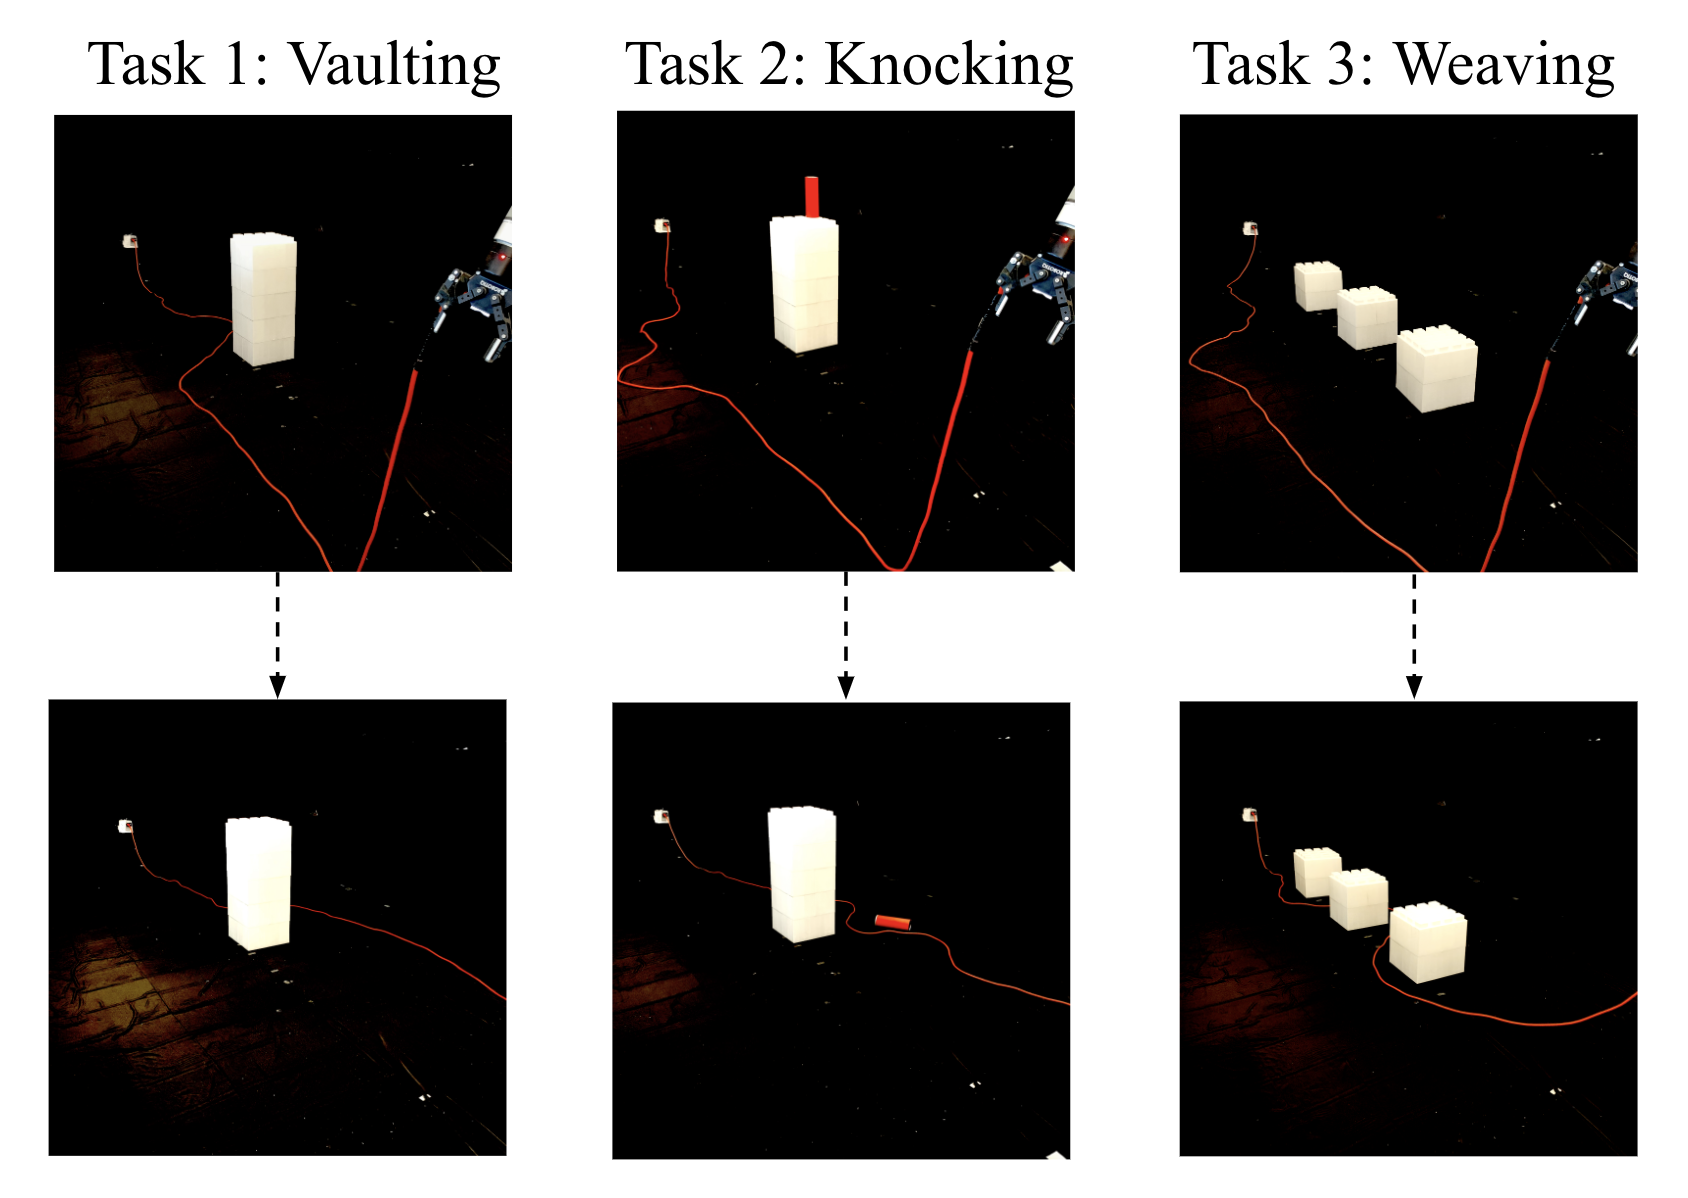
\includegraphics[width=0.48\textwidth]{figures/teaser1.png}
\begin{tikzpicture}[
every node/.style={outer sep=0,node distance=0pt,inner sep=0},
arr/.style={-latex,line width=1pt}]
% IEEE conference format: column width = 3.4in = 244.8pt
% 3 pictures * 80pt = 240pt
% (244.8 - 240)/2 = 4.8/2 = 2.4pt = spacing between pictures
% \node [options] (name) {LaTex Contents of Node};


% \draw [-Triangle,thick] (from_name) -- (to_name); 
% "-Latex" and "-triangle" are arrow types
\node (vs) {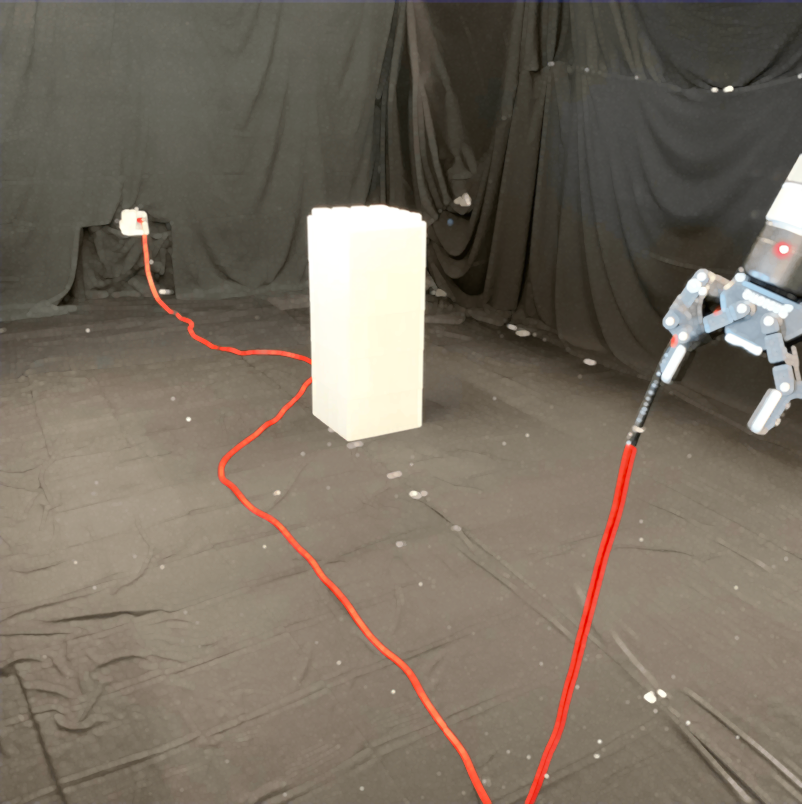
\includegraphics[width=80pt]{figures/teaser_vaulting_start.png}};
\node [right=2.4pt of vs] (ks) {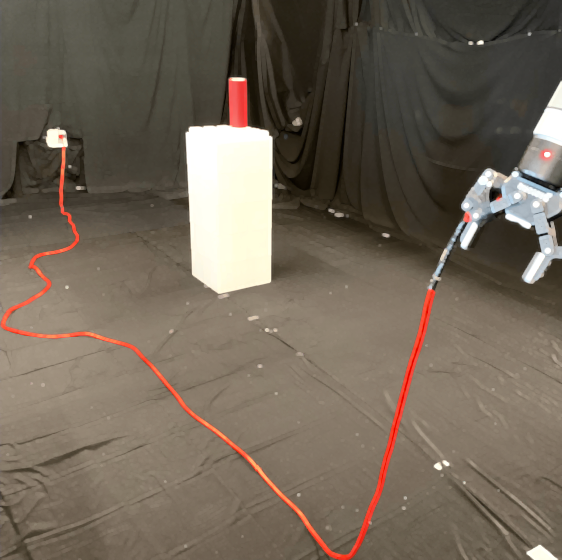
\includegraphics[width=80pt]{figures/teaser_knocking_start.png}};
\node [right=2.4pt of ks] (ws) {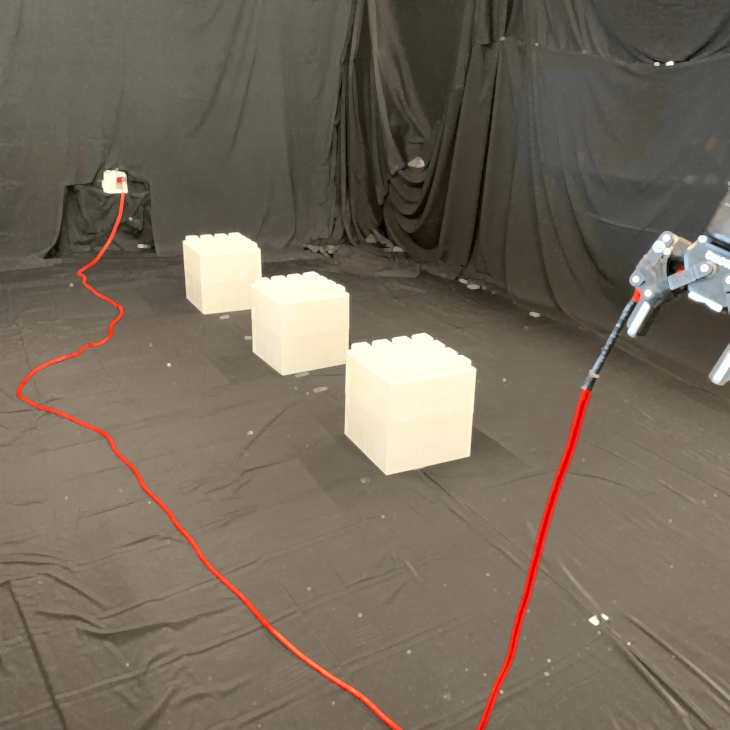
\includegraphics[width=80pt]{figures/teaser_weaving_start.png}};
\node [below=12pt of vs] (ve) {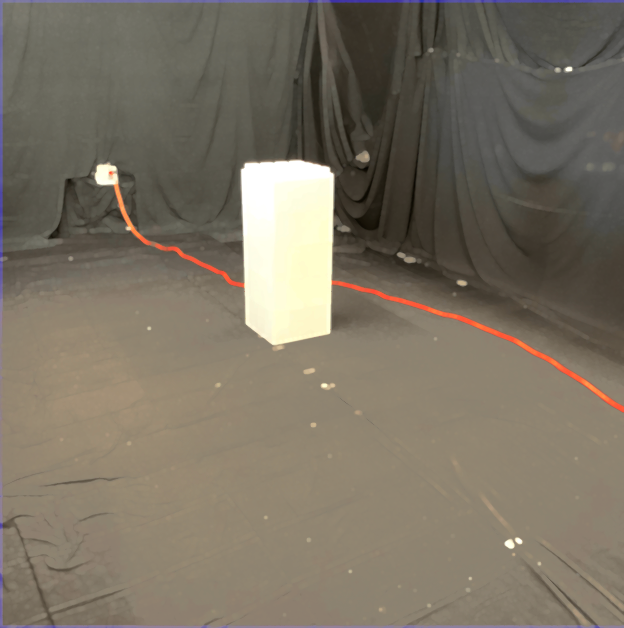
\includegraphics[width=80pt]{figures/teaser_vaulting_end.png}};
\node [below=12pt of ks] (ke) {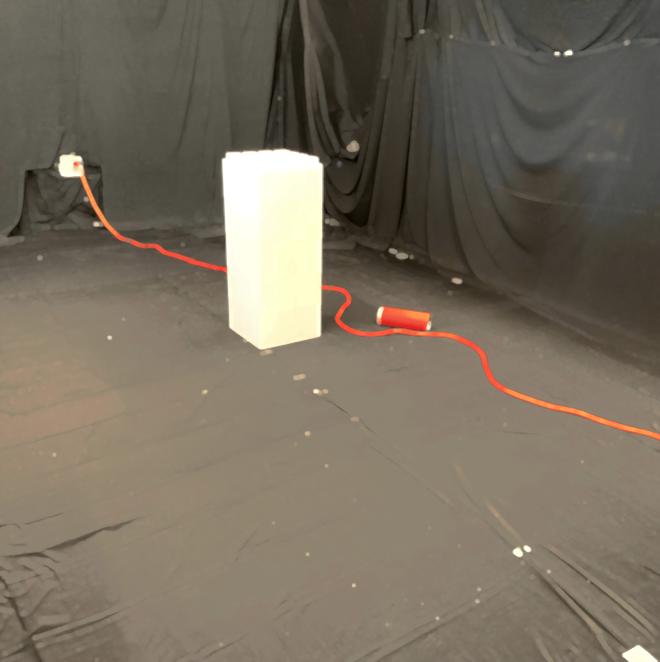
\includegraphics[width=80pt]{figures/teaser_knocking_end.png}};
\node [below=12pt of ws] (we) {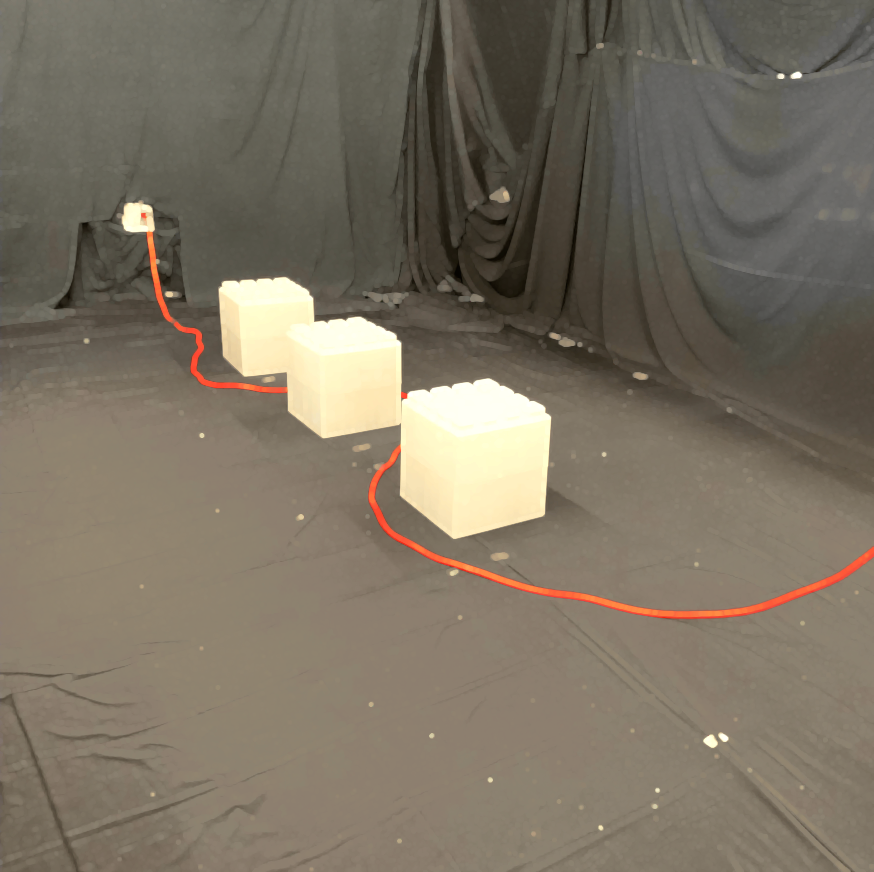
\includegraphics[width=80pt]{figures/teaser_weaving_end.png}};
\draw [arr] (vs) -- (ve);
\draw [arr] (ks) -- (ke);
\draw [arr] (ws) -- (we);
\node [below=4pt of ve] {\footnotesize (a) Task 1: Vaulting};
\node [below=4pt of ke] {\footnotesize (b) Task 2: Knocking};
\node [below=4pt of we] {\footnotesize (c) Task 3: Weaving};
\end{tikzpicture}
\caption{
\small
Illustration of the 3 tasks: Vaulting, Knocking, and Weaving in real experiments with an orange 18-gauge cable. %The cable is plugged into the wall on one end, and attached to the robot's gripper on the other end.
}
\vspace*{-15pt}
\label{fig:three_tasks}
\end{figure}
To accomplish these tasks, we propose to generate trajectories using a parameterized function. To reduce the complexity of parameterizing actions, we compute minimum-jerk trajectories using DJ-GOMP~\cite{GOMP, DJGOMP} that take as input the apex point in the trajectory.  This point, combined with task-specific starting and ending arm configurations, are used to generate a single high-speed trajectory for a physical UR5 robot. 
\begin{figure}
    \centering
    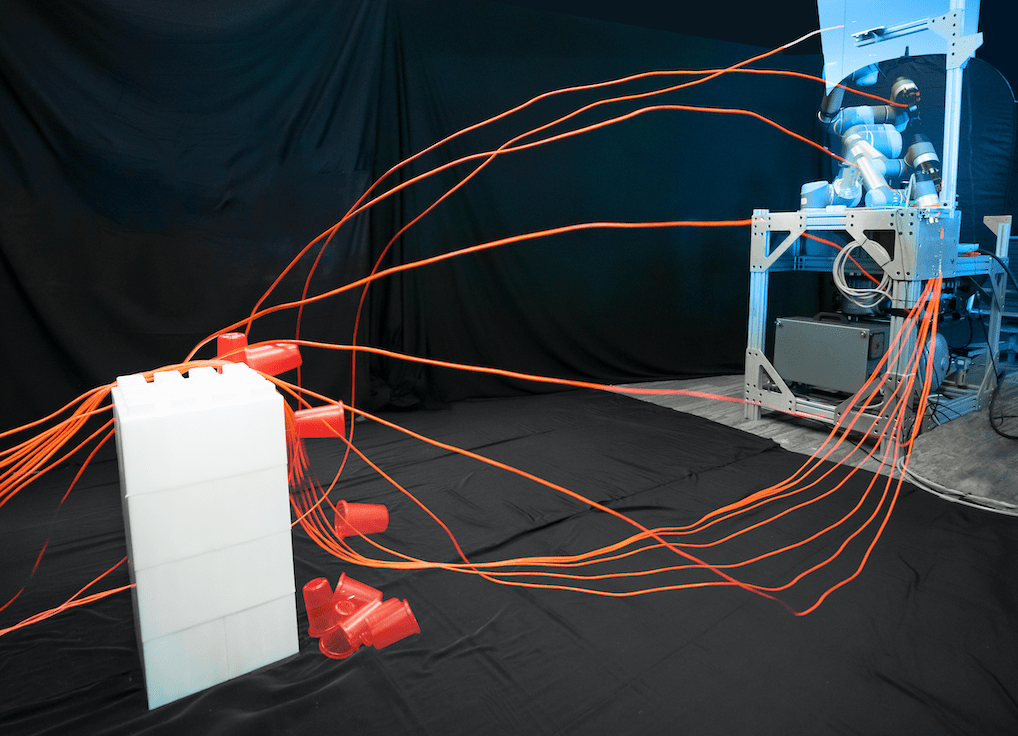
\includegraphics[width=\linewidth]{figures/teaser_new1.png}
    \caption{Long exposure photo of a UR5 robot dynamically manipulating an orange cable fixed at one end (far left) to knock the red target cup off the white obstacle using the learned 3d apex point and minimum-jerk robot trajectory.}
    \label{fig:teaser_new}
    \vspace*{-20pt}
\end{figure}
We present a self-supervised deep imitation learning pipeline that learns to predict the apex point given target positions. Using a simulator we develop for vaulting, with a simulated UR5, we obtain an example action that completes the vaulting task. For any of the three tasks in the real world (see Fig.~\ref{fig:teaser_new}), we then have the physical UR5 continually execute actions based on the action computed in simulation, with noise added to increase dataset diversity. While the robot performs actions, one end of the cable is attached to its gripper, and the other is fixed to a wall. (Hereafter, we use \emph{cable} to refer to any 1D deformable object with low stiffness, such as ropes, cords, and strings.) This process results in a self-supervised procedure for collecting a large dataset. We use the resulting data to train a deep neural network policy to predict an action (i.e., the apex point) given a target position. %The physical experiments setup is shown in Fig.\ref{fig:teaser_new}.
%The system learns using physical trials on a UR5 robot. 

This paper contributes:
\begin{enumerate}
    \item Three novel dynamic cable manipulation tasks: vaulting, knocking, and weaving.
    \item INDy, a self-supervised framework for collecting data and learning a dynamic manipulation policy using parameterized minimum-jerk trajectories.
    \item A simulation platform to experiment with novel tasks and policy learning.
    \item Physical experiments evaluating the policies with a UR5 robot on 5 different cables.
\end{enumerate}


%While humans often accomplish such motions, it is difficult for a robot to generate a feasible trajectory to accomplish this task.
% The key notion we tackle in this paper making the rope manipulation dynamic---with few swift motions of a its manipulator arm a robot accomplishes a task.  We contrast this to prior work that explored quasi-static manipulation of cables in a 2D space, such as knot-tying~\cite{knot_planning_2003, nair_rope_2017}, shape-matching~\cite{nair_rope_2017,yan2020learning} and untangling~\cite{rope_untangling_2013,grannen2020untangling}, few attempt to manipulate cables dynamically in a full 3D space. \jeffi{TODO: reword to place dynamic manipulation in context.}
%To reduce increase the repeatability of actions, we reset the cable each time by pulling it taut and slowing dropping it before each dynamic motion.
%and does not explicitly model cable dynamics (see Section~\ref{sec:method} for details). To minimize the damage to the robot, we generate a trajectory defined by those three points (start, learned 3D apex point, and end) with minimal jerk.

\section{Related Work}

Manipulation of 1D deformable objects has applications in surgical suturing~\cite{schulman_case_study_2013,suturing_autolab_2016}, knot-tying~\cite{van_den_berg_2010,case_study_knots_1991,knot_planning_2003,tying_precisely_2016}, untangling ropes~\cite{rope_untangling_2013,grannen2020untangling,tactile_cable_2020}, deforming wires~\cite{wire_insertion_1996,wire_insertion_1997}, and inserting cables into obstacles~\cite{tight_tolerance_insertion_2015}; Sanchez et al.~\cite{survey_2018} provide a survey.

Various approaches have been proposed for quasistatic manipulation of cables, such as using demonstrations~\cite{schulman_isrr_2013,lee_LFD_IROS_2014,seita_bags_2021}, self-supervised learning~\cite{nair_rope_2017,ZSVI_2018, jin2024multi}, model-free reinforcement learning~\cite{lerrel_2020,corl2020softgym, elmquist2022art}, contrastive learning~\cite{yan2020learning, sim2019personalization}, dense object descriptors~\cite{priya_2020, eisner2022flowbot3d, pan2023tax}, generative modeling~\cite{wang_visual_planning_2019, avigal20206, avigal2021avplug}, and state estimation~\cite{state_estimation_LDO, zhang2020dex, zhang2021robots, zhang2023flowbot++, yao2023apla}. These prior works generally assume quasistatic dynamics to enable a series of small deformations, often parameterized with pick-and-place actions. Alternative approaches involve sliding cables~\cite{one_hand_knotting_tactile_2007,zhu_sliding_cables_2019} or assuming non-quasistatic systems that enable tactile feedback~\cite{tactile_cable_2020, jin2024multi}. This paper focuses on dynamic actions to manipulate cables from one configuration to another, traversing over obstacles and potentially knocking over objects.

More closely related is the work of Yamakawa et al.~\cite{dynamic_knotting_2010,yamakawa2012simple,high_speed_knotting_2013,one_hand_knotting_tactile_2007, zhang2016health, devgon2020orienting, lim2021planar, lim2022real2sim2real} that focuses on dynamic manipulation of cables using robot arms moving at high speeds, enabling them to model rope deformation algebraically under the assumption that the effect of gravity is negligible. They show impressive results with a single multi-fingered robot arm that ties knots by initially whipping cables upwards. Because we use fixed-endpoint cables moving at slower speeds, the forces exerted on the rope by gravity and the fixed endpoint prevent us from performing knot ties. %assuming a model where each rope joint follows the robot motion with constant time-delay, as in Yamakawa~et~al. Instead, we use a learning-based method and do not use specialized end-effectors.
Kim and Shell~\cite{kim2016using, shen2024diffclip} use a small-scale mobile robot with a cable attached as a tail to manipulate small objects by leveraging inter-object friction to drag or strike the object of interest. While their work aims to tackle dynamic cable control, it relies heavily on physics models for motion primitives that are only applicable to dragging objects via cables, and uses a RRT-based graph search algorithm to address the stochasticity in the system. Other studies have developed physics models to analyze dynamic cable motion. For example, Zimmermann et al.~\cite{zimmermanndynamic} use the finite-element method to model elastic objects for dynamic manipulation of free-end deformable objects, and Gatti-Bonoa and Perkins~\cite{fly_fishing_2004} and Wang and Wereley~\cite{wang2011analysis} analyze fly fishing rod casting dynamics. We focus on fixed-end cable manipulation and do not attempt to model cable physics, and we aim to control cables dynamically via vaulting, knocking, and weaving, and cannot rely on the same dragging motion primitives as in Kim and Shell~\cite{kim2016using}.

We propose an approach that is related to TossingBot~\cite{zeng_tossing_2019} where a robot learns to toss objects to target bins. TossingBot uses RGBD images and employs fully convolutional neural networks~\cite{fcn_2015} to learn dense, per-pixel values of tossing actions, and learns a residual velocity of tossing on top of a physics model in order to jointly train a grasping and tossing policy through trial and error. We take a similar approach in dynamically manipulating by reducing the learning process to learn only the joint angles of the apex of the motion. We do not rely on a physics model of the dynamic manipulation motion, and instead, leverage a quadratic programming-based motion-planning primitive to generate a fast ballistic motion that minimizes the jerk while moving through the learned apex point.

\section{Problem Definition}
Given a manipulator arm holding one end of a cable with the other end fixed (e.g., plugged into a wall), the objective is to compute and execute a single high-speed arm motion from a fixed far-left starting location, to a fixed far-right ending location that moves the cable from an initial configuration to a configuration that matches a task-dependent goal constraint.

Let $s \in \mathcal{S}$ be the configuration of the cable and task-specific objects, including obstacles or targets, where $\mathcal{S}$ is the configuration space.
%Let $\mathcal{E}$ be the obstacle environment.
Since $\mathcal{S}$ is infinite-dimensional, we consider observations of the state, and focus on tasks for which the observations are sufficient to capture progress.  Let $o \in \mathcal{O}$ be the observation, where $\mathcal{O}$ is the observation space and $f_c : \mathcal{S} \rightarrow \mathcal{O}$ map a state to an observation (e.g., via a camera view).
Let $\tau_a \in \mathcal{A}$ be the action the manipulator arm takes, where $\tau_a$ is a complete open-loop trajectory and $\mathcal{A}$ is the action space.
Let $f_\mathcal{S} : \mathcal{S} \times \mathcal{A} \rightarrow \mathcal{S}$ be the stochastic state transition function of the cable.

% REMOVED PER KG 3/25
%The observation space needs to encode sufficient information for the policy to infer actions, such as the dimension and location of the target object and/or the obstacle.  Thus, in our problem, a camera positioned slightly above the manipulator arm should contain sufficient information to cover the minimum observation space.
%Thus, $\mathcal{O} = \mathbb{R}^{w\times h\times 3}$, where $w \times h$ are the dimensions of an RGB image in our experiments.

Formally the objective is: for each task $i \in \{ \mathrm{vaulting},\allowbreak \mathrm{knocking},\allowbreak \mathrm{weaving} \}$, to learn a task-specific policy $\pi_i : \mathcal{O} \rightarrow \mathcal{A}$, that when given the observation $o_0 = f_c(s_0)$ of 
an initial configuration $s_0 \in \mathcal{S}$ and a goal set of observations $\mathcal{O}_\mathrm{goal} \subset \mathcal{O}$, computes an action $\tau_a \in \mathcal{A}$ such that $f_c(f_\mathcal{S}(s_0,\tau_a)) \in \mathcal{O}_\mathrm{goal}$. For each task, we define the goal set in terms of constraints, such as requiring an observation with the cable on the right side of an obstacle (Fig.~\ref{fig:three_tasks}~(a)).
\begin{figure}[t]
\vspace*{5pt}

\center
%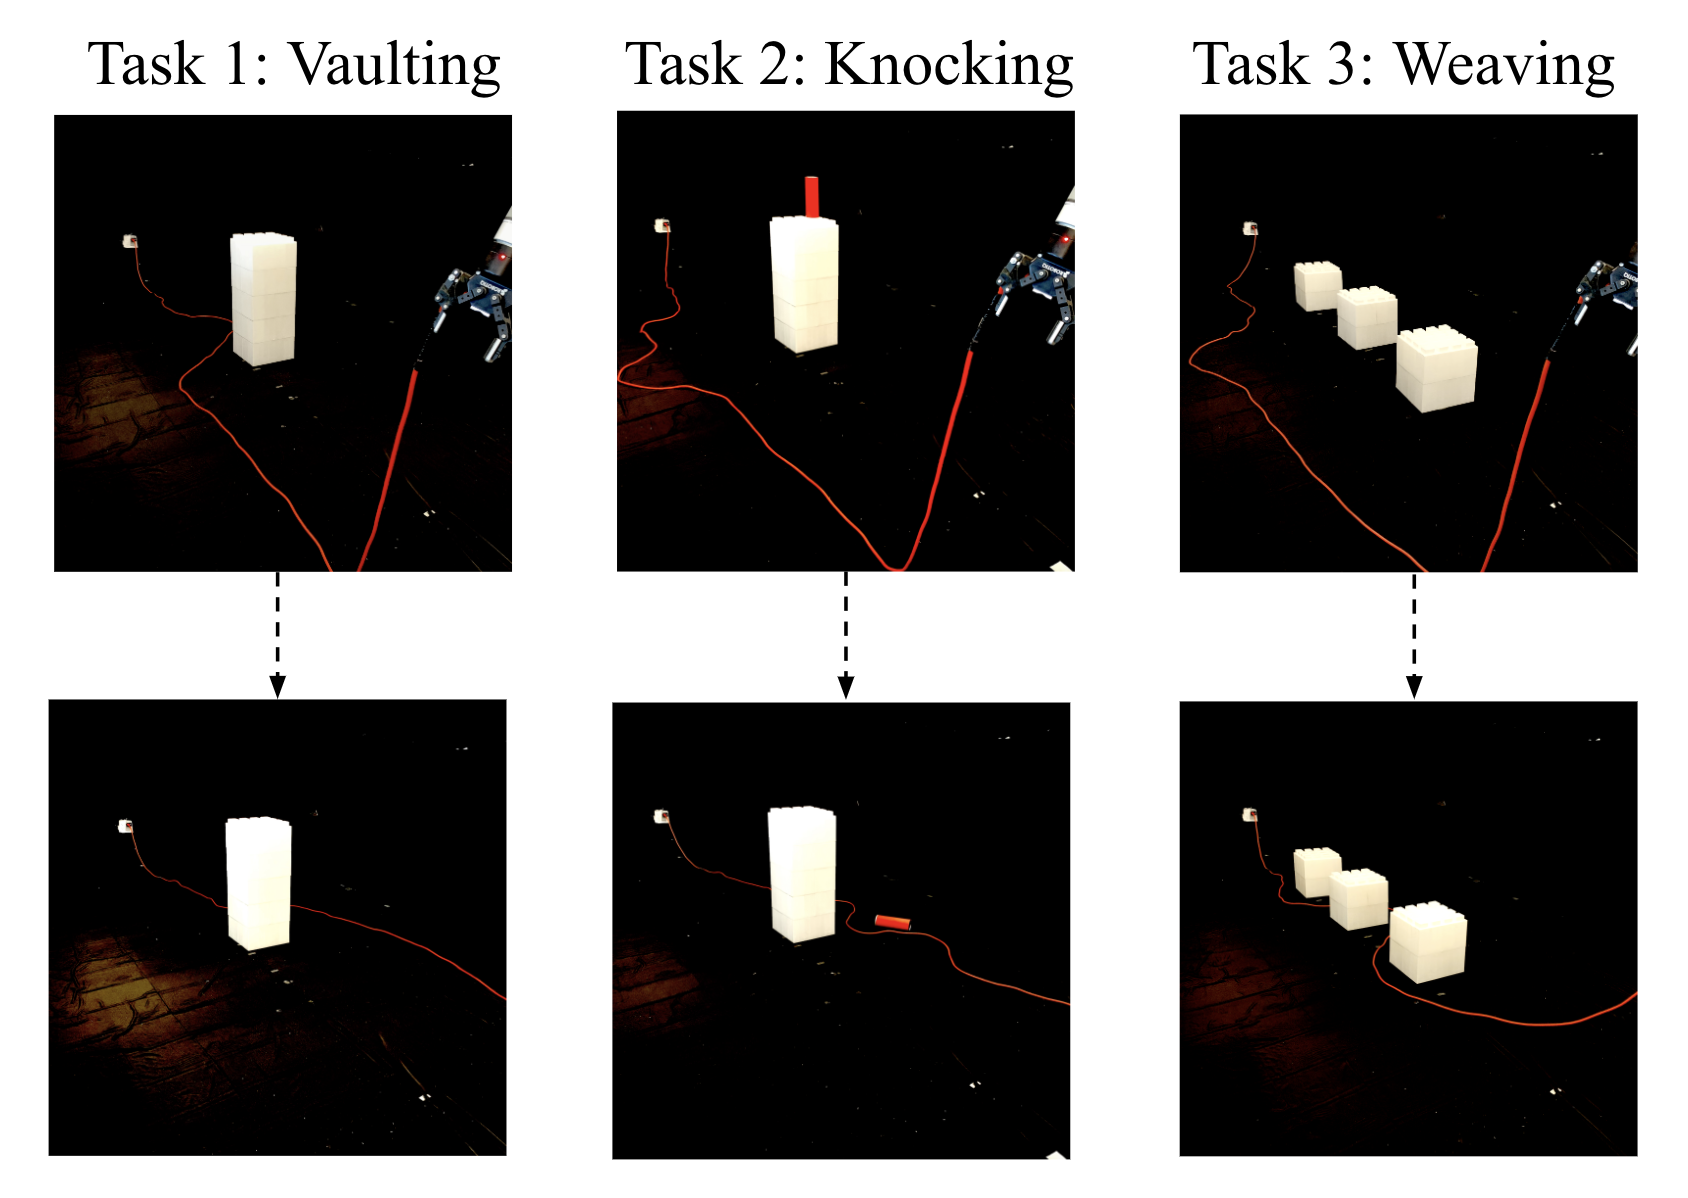
\includegraphics[width=0.48\textwidth]{figures/teaser1.png}
\begin{tikzpicture}[
every node/.style={outer sep=0,node distance=0pt,inner sep=0},
arr/.style={-latex,line width=1pt}]
% IEEE conference format: column width = 3.4in = 244.8pt
% 3 pictures * 80pt = 240pt
% (244.8 - 240)/2 = 4.8/2 = 2.4pt = spacing between pictures
% \node [options] (name) {LaTex Contents of Node};


% \draw [-Triangle,thick] (from_name) -- (to_name); 
% "-Latex" and "-triangle" are arrow types
\node (vs) {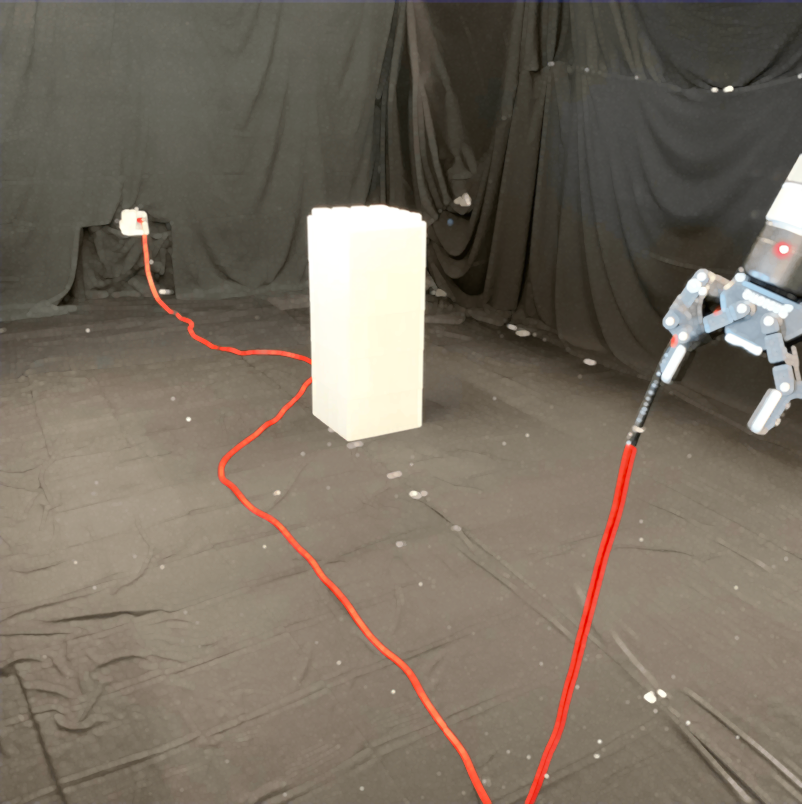
\includegraphics[width=80pt]{figures/teaser_vaulting_start.png}};
\node [right=2.4pt of vs] (ks) {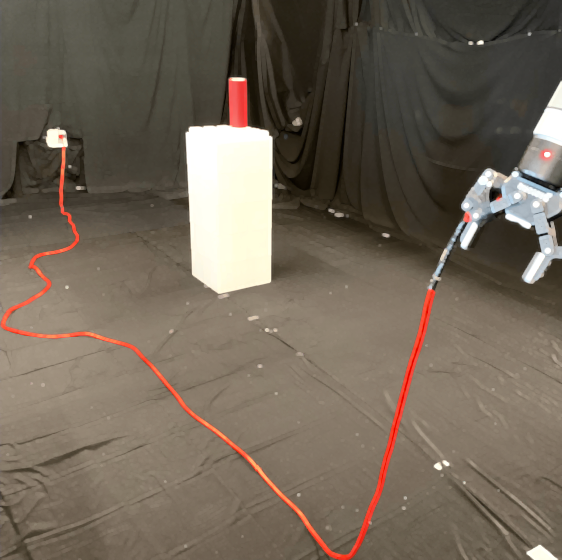
\includegraphics[width=80pt]{figures/teaser_knocking_start.png}};
\node [right=2.4pt of ks] (ws) {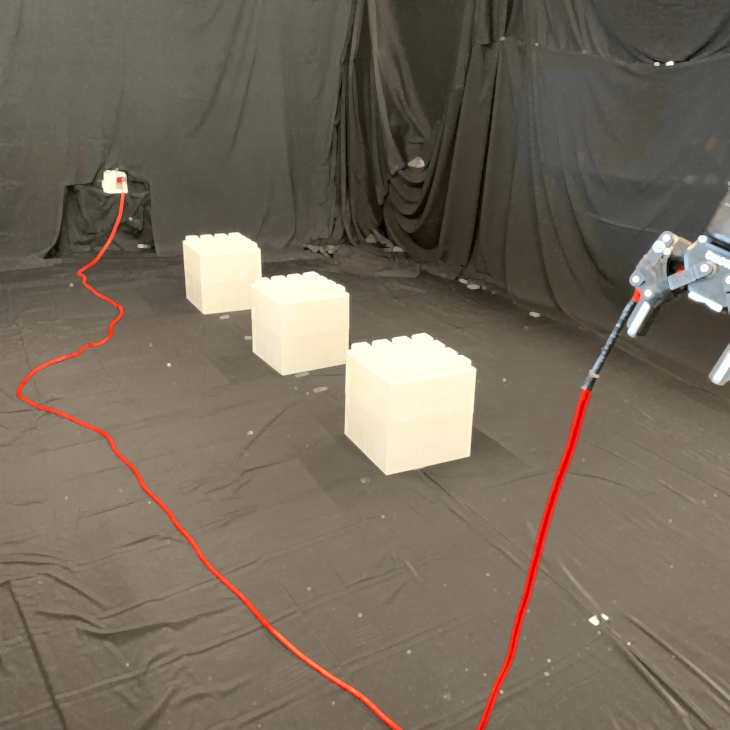
\includegraphics[width=80pt]{figures/teaser_weaving_start.png}};
\node [below=12pt of vs] (ve) {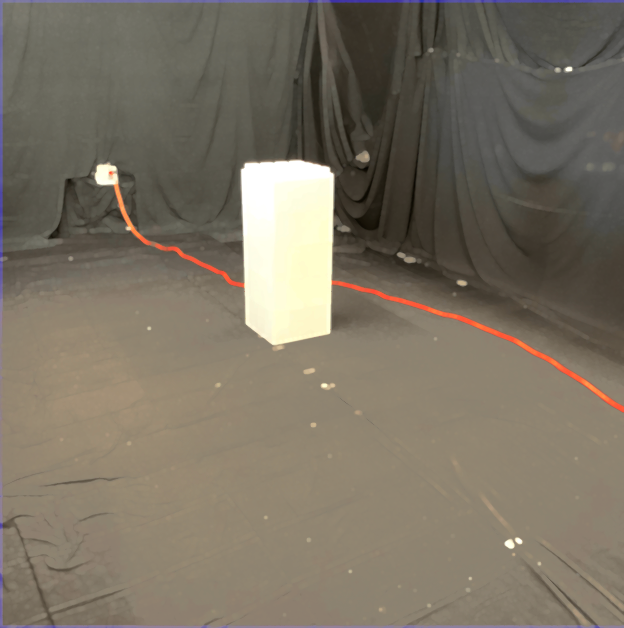
\includegraphics[width=80pt]{figures/teaser_vaulting_end.png}};
\node [below=12pt of ks] (ke) {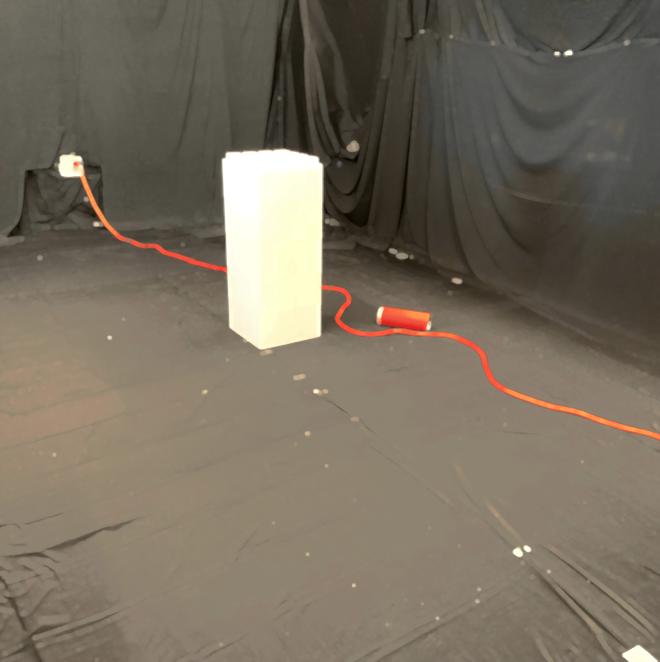
\includegraphics[width=80pt]{figures/teaser_knocking_end.png}};
\node [below=12pt of ws] (we) {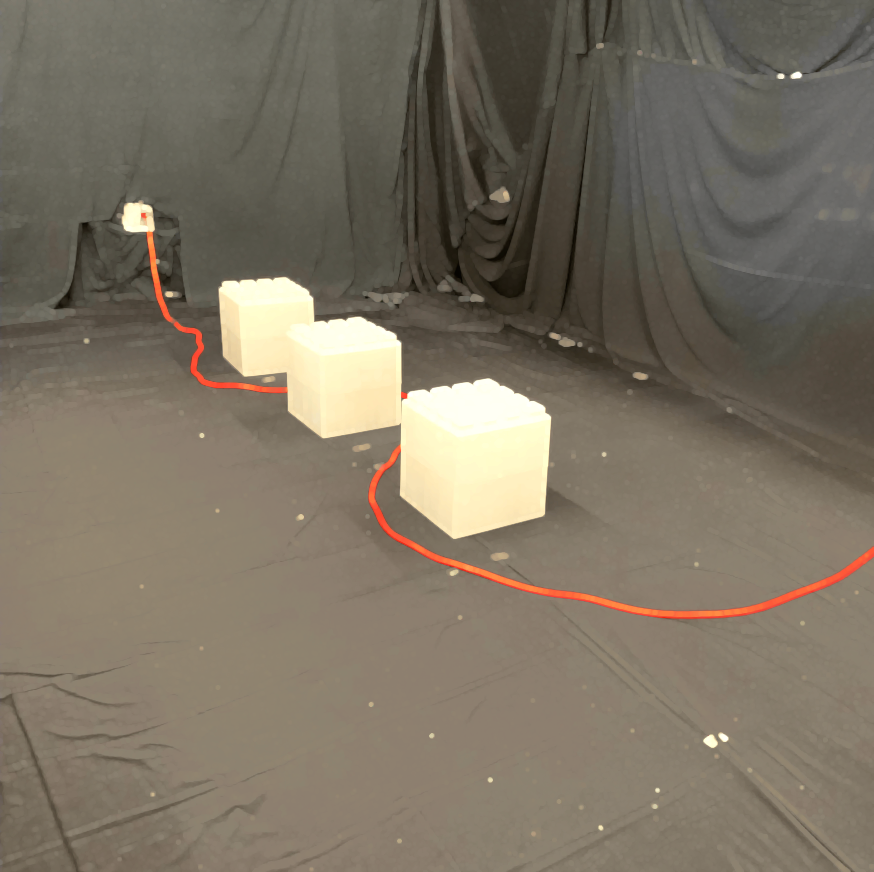
\includegraphics[width=80pt]{figures/teaser_weaving_end.png}};
\draw [arr] (vs) -- (ve);
\draw [arr] (ks) -- (ke);
\draw [arr] (ws) -- (we);
\node [below=4pt of ve] {\footnotesize (a) Task 1: Vaulting};
\node [below=4pt of ke] {\footnotesize (b) Task 2: Knocking};
\node [below=4pt of we] {\footnotesize (c) Task 3: Weaving};
\end{tikzpicture}
\caption{
\small
Illustration of the 3 tasks: Vaulting, Knocking, and Weaving in real experiments with an orange 18-gauge cable. %The cable is plugged into the wall on one end, and attached to the robot's gripper on the other end.
}
\vspace*{-15pt}
\label{fig:three_tasks}
\end{figure}

%Let $a \in \mathcal{A}$ be the action the manipulator arm takes.  Let $f_\mathcal{S}: \mathcal{S} \times \mathcal{A} \rightarrow \mathcal{S}$ be stochastic state transition function of the cable. As $\mathcal{S}$ is the infinite-dimensional configuration space of the cable, we instead rely on observations $o \in \mathcal{O}$ of the cable to define the start and goal state of the problem. Let $f_c : \mathcal{S} \rightarrow \mathcal{O}$ be a function that maps the cable's state to an observation of that state (e.g., via a camera view).  Let $T$ be the horizon of our control problem. Let $f_\mathcal{S} : \mathcal{S} \times \mathcal{A}^{T} \rightarrow \mathcal{S}$ be the stochastic open-loop state transition function of the cable after applying an actions sequence of length $T$.
%We denote states as $s_t$, observations as $o_t$, and actions as $a_t$. We denote the unknown, stochastic state transition function of the rope object as $f(s_t, a_t)$.



Since the action space $\mathcal{A}$ is also infinite-dimensional, we define a parametric trajectory function $f_{\mathcal{A}_i} : \mathbb{R}^3 \rightarrow \mathcal{A}$, that, when given an apex point, computes complete arm trajectory. While the exact function is a design choice,
we propose that the function should have
the following features: the arm motions are fast enough to induce a motion over the length of the cable, the apex point of the motion can be varied based on an $\mathbb{R}^3$ input,  the other points in the trajectory vary smoothly through the apex, and the motions are kinematically and dynamically feasible. This converts the problem to learning $\hat\pi_i : \mathcal{O} \rightarrow \mathbb{R}^3$, where $\mathcal{O}$ contains position and dimension information, such that for the action $a \in \mathbb{R}^3$ computed by the policy, $f_c(f_\mathcal{S}(s_0, f_{A_i}(a))) \in \mathcal{O}_\mathrm{goal}$.


% This is now stated in the first paragraph of the problem definition:
%We assume the manipulator arm's end-effector holds one end of the LDO, and the other end of the LDO is fixed (e.g., a power cord is plugged into the wall).
%For this work, we do not consider state feedback, and instead focus on the computation of an open-loop motion for the manipulator arm.%, so the learned policy is a shooting-method-based policy. 

% Given the initial configuration of the cable $s^r_0$ and the obstacle configuration $s^o_0$, the robot observes $o_0 = f_c( s^r_0, s^o_0 )$.
% For each task, we are given a goal set of terminal configurations $\mathcal{S}_g \subset \mathcal{S}$. For example, in the snapping task, $\mathcal{S}_g$ is a set of final configurations of the cable that knock the object over by snapping it. Therefore, we use $o_0$ and $\mathcal{S}_g$ as the input to the system. We wish to learn a policy $\pi_\theta$ such that: \harry{TODO: prof. G said Sg does not need to be specified. How do we fix this?}
% \[
% s^r_T = f_{\mathcal{S}}(s^r_0, a_{0:T-1}\sim \pi_\theta(a|o_0))\in \mathcal{S}_g
% \]
% \[
% \exists s^r_i \in \{s^r_0, ..., s^r_T\}, s^r_i = s_g
% \]
% where $s_g$ is varied for each task. For example, in the snapping task, $s_g$ is a state where the cable intersects the target object.
% In the system, policy $\pi_\theta$ is a stochastic policy that outputs a vector representing joint angles of the robot, so we are not inferring the whole trajectory of the motion, but learning a low-dimensional parameterization of a trajectory.
% %\jeffi{This is sort of previewing that we are not learning a trajectory, but a low-dimensional parameterization of a trajectory.  We may wish to be explicit on this point here.  I think though, its belongs more to the method description.} \harry{Added}
% \harry{TODO: Need to update the equation above to show that we apply this action T times.}
% Daniel: figure should take up the full width to be clearer to readers.
% \usepackage{subcaption}
% \begin{figure}[H]
% \begin{subfigure}{.25\textwidth}
%   \centering
%   % include first image
%   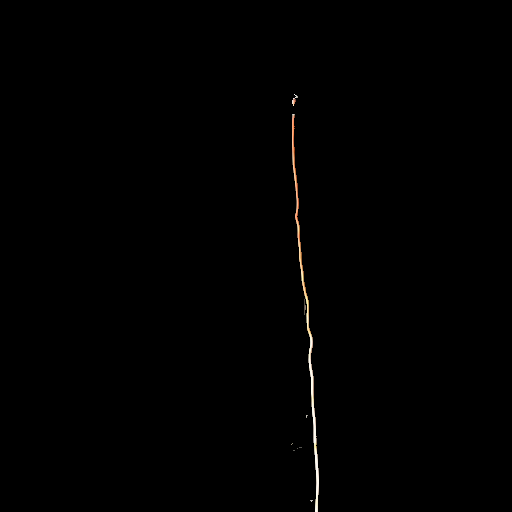
\includegraphics[width=.6\linewidth]{figures/taut_seg.png}  
%   \caption{Taut rope after reset}
%   \label{fig:sub-first}
% \end{subfigure}
% \begin{subfigure}{.25\textwidth}
%   \centering
%   % include second image
%   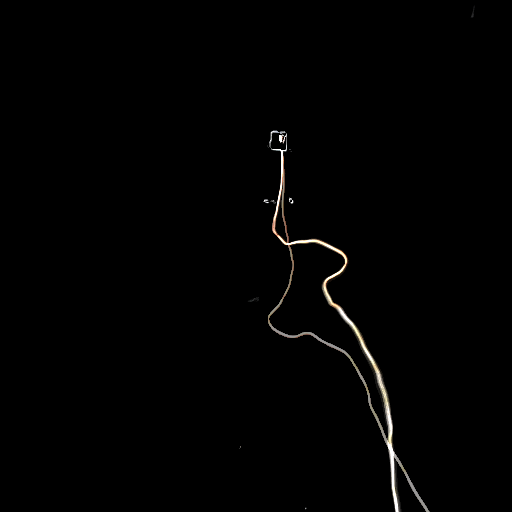
\includegraphics[width=.6\linewidth]{figures/repeat2.png}  
%   \caption{Repeatability across 20 trials}
%   \label{fig:sub-second}
% \end{subfigure}
% \caption{\textbf{Left: }the starting state of the rope is almost straight after being reset before each action begins. \textbf{Right: }overlaid image of 20 ending states of the rope after applying the same left-to-right whipping motion for 20 times given the same reset. The ending states of the rope are almost identical across 20 trials, with 1 outlier, so each action is repeatable. \harry{TODO: Re: Yes they are extremely similar. There is a kinda blurry region in the middle tho, and I did 10 more trials and had one outlier.} \jeffi{Random idea: Would it be possible to have each trial have a different color?  So we would see sort of  rainbow blob or cables?}}
% \label{fig:repeat}
% \end{figure}

\begin{figure}[t]
    \vspace*{5pt}
    \centering
    % \begin{tabular}{c@{\hspace{1.5pt}}c@{\hspace{1.5pt}}}
    %\subfloat[Ending states without reset]{%
    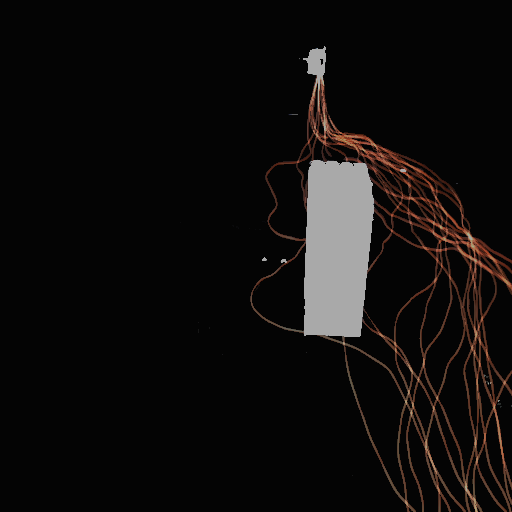
\includegraphics[height=122pt]{figures/unrepeata.png}%}%
    \hfill
    %\subfloat[Ending states with reset]{%
    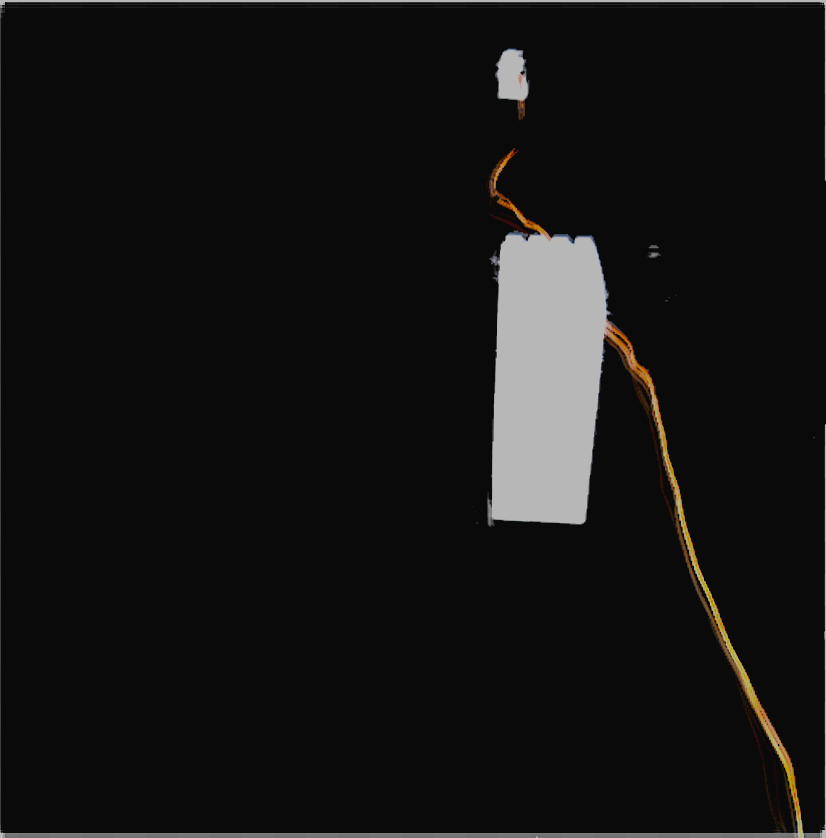
\includegraphics[height=122pt]{figures/repeat4a.png}%}
    % \end{tabular}
    \caption{\textbf{Repeatability without (left) and with (right) taut-pull reset.} 
    Both images show an overlay of 20 ending cable configurations after sequentially applying the same left-to-right vaulting trajectory 20 times. \textbf{Left: }without applying resets before the motion, there is high variation in ending configurations.  \textbf{Right: }resetting the cable via a taut-pull before the motion results in nearly identical configurations across 20 left-to-right attempts.}% The vaulting actions are surprisingly repeatable with reset.}
    %\vspace*{-10pt}
    \label{fig:repeat}
\end{figure}


%\section{Hypothesis}

{\color{red} TODO: incoporate KG feedback from 10/29.  TODO: consider incorporating aspects of the hypothesis throughout appropriate sections.}

% From observing humans whipping a fixed-endpoint cable from left to right, we see that the trajectory of the cable's held end is a smooth curve that resembles a arc where the first half of the arc moves the held end up and the second half moves the held end down. Furthermore, we observe that even when humans whip the fixed-endpoint cable with a small reach, the middle segment of the cable often travels a much longer distance than the reach of the human arm. We can model this phenomenon using the following physical property: the speed of a wave $v$ along an unconstrained cable can be calculated as $v=\sqrt{T_c/\mu}$, where $T_c$ is the tension in cable and $\mu$ is the mass per unit length. When whipping an unconstrained cable homogeneous in mass, assuming minimal drag and friction, the velocity along the cable should be constant. In reality, when we are using a finite-length cable, the energy loss in drag and friction should be minimal. However, since we fix the endpoint of the cable, the endpoint's velocity is constrained to be 0, which will propagate the kinetic energy that should have been dissipated from the endpoint into the cable, making the middle segments of the cable travel faster, thus travelling a longer distance than the held end of the cable does in a given period of time. With this observation, we can whip the cable to long distances with a robot arm that has a fixed, limited reach. Additionally, at the apex of the motion, the held end experiences a shift in direction, from upwards to downwards, while still maintaining a non-zero horizontal velocity due to inertia. By changing the location of the apex of the whipping motion in space, we are also changing the kinetic energy and gravitational potential energy stored at the apex, thus changing the velocity induced along the cable during the descent part of the motion, varying the landing location of the cable. Thus, by changing the apex of the whipping motion, we can also change the landing location of the cable.
As one end of the cable is fixed and the robot can reset the cable to approximately the same starting state each time, we conjecture that for a reasonable range of motions, the trajectory of the cable can be repeatedly controlled by the trajectory of the robot gripper holding the other end of the cable. Fig.~\ref{fig:repeat} describes experiments on repeatability. The cable can always be reset to a relatively known initial state to the left of the obstacle. %To make the problem tractable and to avoid damage to the robot arm, 

We hypothesize that a minimum-jerk arcing motion defined by 3 points with max velocity at the apex will solve many vaulting problems. We instantiate the initial and final point for the robot at the far left and right of the robot's reachable workspace. The problem now is reduced to finding the apex (mid-point) for the arc and a minimum-jerk trajectory.
An illustration of this three-point arcing motion is shown in Fig.~\ref{fig:3point}. We propose the following procedure to dynamically manipulate the cable: given fixed starting and ending configurations of the robot arm holding the free end of a fixed-endpoint cable, generate a whipping motion by inferring the robot arm configuration at the apex of this whipping motion.
% Since the trajectory of the cable's held end when being whipped is almost arcing, and the robot arm has a fixed maximum reach, we take inspiration from parameterizing a arc of fixed $x$-intercepts and hypothesize that we can fix the starting and ending configurations of the robot arm and control the whipped cable by varying the robot configuration at the apex point of this semi-arcing motion. Besides validating the hypothesis in theory using the aforementioned energy view, we also validate the hypothesis in simulation by comparing the three-point arc model with different models. 

% We use simulation to evaluate the hypothesis on the 3-point dynamic motion, and to find a feasible base policy $\pi_\beta$ for data collection. Using simulation enables fast resetting to efficiently evaluate the qualitative behavior of multiple base policies. For simulation, we use Blender~\cite{blender}, because it has previously worked reasonably well for manipulating 1D~\cite{priya_2020} and 2D structures~\cite{descriptors_fabrics_2020}. Blender's keyframe feature allows us to specify robot configurations at certain animation frames, with the robot motion between keyframes being automatically interpolated. Additionally, Blender has an easy to use Python API, and its built-in rendering engine Eevee supports ray-tracing, making rendering fast on GPUs.

% To model cables in simulation, we use a Featherstone~\cite{featherstone1984robot} rigid-body simulator from BulletPhysics via Blender. Cables are implemented as a series of small capsule links connected by spring and torsional forces. We hand-tune the spring constants, torsional stiffness, and damping coefficients to make the simulated cable behave physically similar to a power cord. Specifically, in Blender, we use a torsional stiffness value of 1, a twist damping value of 0.9, a spring stiffness value of 40, and a spring damping value of 0.5.

% Using this setup, we compare the three-point arc model with different models. First, we tried regressing both apex point location and velocity explicitly, and found that regressing velocity did not improve the success rate of the vaulting task. We have also tried interpolating a straight-line motion between the points without making it arcing and found that the discontinuity in the middle causes the robot to come to a complete stop at the apex, thus reducing the energy stored for the cable to move fast enough. 


% We find the starting and ending configurations of the robot by moving the robot arm in free space to obtain the maximum left-to-right reach without violating safety constraints (e.g. hitting the camera mount). 

% We model the robot configuration at the apex as a 3D vector representing the three joint angles of the robot at the apex: $a_t = \langle \phi_{\rm base}, \phi_{\rm shoulder}, \phi_{\rm elbow} \rangle\in \mathbb{R}^3, \;\forall{t}\in [0,\dots T-1]$. In vaulting and knocking, $T=2$, and in weaving, $T=3$. 
\section{Method}
\label{sec:method}

\newcommand{\Tj}[1]{\includegraphics[width=28mm, clip]{figures/#1}}

% \input{method_overview}

%To compute fast motions for a robot arm to dynamically manipulate a cable to accomplish a task, we
We propose a deep-learning system that takes as input an image, and produces a sequence of timed joint configurations; when the robot to follows the motion, it results in the dynamic manipulation of a cable that accomplishes the task.
%In this section, we describe the action formulation, the training procedure, the trajectory generation algorithm, and the setup for simulated and real experiments. 

\begin{algorithm}[t!]
\caption{\small Iterative traiNing for Dynamic manipulation (INDy)}
\small{
\begin{algorithmic}[1]
\algsetup{linenosize=\small}

\label{alg:whip}
\REQUIRE Base action of task $i$ $a_{\beta, i}$, a task-trajectory function $f_{\mathcal{A}_i}$, a goal observation set $\mathcal{O}_\mathrm{goal}$, number of data points $N$, the task's time horizon $T$.
\STATE Empty dataset $\mathcal{D} = \{\}$.
\FOR{$t$ $\in \{1 \ldots N\}$}
    \STATE Randomize environment (obstacle size and location)
    \STATE Pull taut to reset to cable's state (updates $s_t$)
    \STATE $o_t \leftarrow f_c(s_t)$ \COMMENT{record initial observation}
    \STATE Set starting action $a_{0:T} = a_{\beta, i}$
    %\WHILE{not successful}
    \LOOP
        \STATE $\tau_a \leftarrow f_{\mathcal{A}_i}(a_{0:T})$ \COMMENT{compute trajectory}
        \STATE execute $\tau_a$ on the robot (updates $s_t$)
        %\STATE Rollout actions $a_{0:T}$, record observation $o_T$
        \IF{$f_c(s_t)\in\mathcal{O}_\mathrm{goal}$}
            \STATE \textbf{break} \COMMENT{success observed}
        \ENDIF
        \STATE Pull taut to reset to cable's state (updates $s_t$)
        \STATE $a_{0:T} \leftarrow a_{0:T} + \mathrm{(random\;noise)}$
    %\ENDWHILE
    \ENDLOOP
    \STATE $\mathcal{D} \longleftarrow \mathcal{D} \cup \{(o_t, a_{0:T})\}$ 
\ENDFOR
\STATE Train policy $\pi_i(a|o)$ with $\mathcal{D}$ to minimize Eq.~\ref{eq:loss}.
\RETURN Trained policy for task $i$, $\pi_i(a|o)$
\end{algorithmic}
}
\end{algorithm}
%% OLDER WAY BELOW
%\begin{algorithm}[t!]
%\caption{Self-Supervised Training Procedure}
%\small{
%\begin{algorithmic}[1]
%\algsetup{linenosize=\small}
%
%\label{alg:whip}
%\REQUIRE Base policy of task $i$ $\pi_{\beta, i}(a|o)$, a task-trajectory function $f_{\mathcal{A}_i}$, a goal observation set $\mathcal{O}_\mathrm{goal}$, number of data points $N$, the task's time horizon $T$.
%\STATE \texttt{obs = []}, \texttt{acts = []}
%\FOR{$t$ $\in \{1 \ldots N\}$}
%    \STATE Randomize env (obstacle size and location)
%    \STATE Pull taut to reset to cable's state (updates $s_t$)
%    \STATE $o_t \leftarrow f_c(s_t)$ \COMMENT{record initial observation}
%    \STATE \texttt{obs}.append$(o_t)$
%    \STATE Set base action $a_{0:T} \sim \pi_{\beta, i}(a|o_t)$
%    %\WHILE{not successful}
%    \LOOP
%        \STATE $\tau_a \leftarrow f_{\mathcal{A}_i}(a_{0:T})$ \COMMENT{compute trajectory}
%        \STATE execute $\tau_a$ on the robot (updates $s_t$)
%        %\STATE Rollout actions $a_{0:T}$, record observation $o_T$
%        \IF{$f_c(s_t)\in\mathcal{O}_\mathrm{goal}$}
%            \STATE \textbf{break} \COMMENT{success observed}
%        \ENDIF
%        \STATE Pull taut to reset to cable's state (updates $s_t$)
%        \STATE $a_{0:T} \leftarrow a_{0:T} + \mathrm{(random\;noise)}$
%    %\ENDWHILE
%    \ENDLOOP
%    \STATE \texttt{acts}.append($a_{0:T}$)
%\ENDFOR
%\STATE Form training data $\mathcal{D} = \{\mathcal{O}:\texttt{obs},\; \mathcal{A}:\texttt{acts}\}$.
%\STATE Train policy $\pi_i(a|o)$ with $\mathcal{D}$ to minimize $\mathcal{L}_{\mathrm{MSE}} = \frac{1}{2}||\hat{a}_{0:T} - a_{0:T}||_2^2$ where $\hat{a}_{0:T}\sim \pi_i(a|o_t)$, using the reparameterization trick~\cite{vae}.
%\RETURN Trained policy for task $i$, $\pi_i(a|o)$
%
%\end{algorithmic}
%}
%\end{algorithm}
\subsection{Hypothesis}

\paragraph*{Repeatability} A cable with fixed length is attached to the wall and with a gentle pull, the robot can reset the cable to a consistent starting state before each motion.  The same arm trajectory will result in a similar end configuration of the cable (Fig.~\ref{fig:repeat}).

\paragraph*{Parameterized Trajectory Function} We hypothesize that a high-speed minimum-jerk ballistic manipulator-arm motion can solve many left-to-right vaulting problems by varying the midpoint location in $(x,y,z)$ (Fig.~\ref{fig:motion_and_floor}~left).  This reduces the problem to finding which $\mathbb{R}^3$ input to a trajectory function $f_{\mathcal{A}_i}$ solves the task.  This is akin to the $\mathbb{R}^2$-regression TossingBot~\cite{zeng_tossing_2019} uses to throw objects.

\subsection{Deep-Learning Training Algorithm} % Was: {Data Collection and Training Procedure}
\label{sec:deep_alg}


We propose a self-supervised training algorithm, INDy (Alg.~\ref{alg:whip}), to learn a policy $\pi_i$ for task $i$. The main inputs are:
a base action for the task $a_{\beta,i}$, 
a task-trajectory function $f_{\mathcal{A}_i}$, and
a goal observation set $\mathcal{O}_\mathrm{goal}$.

To train the policy, INDy
%The training process
first forms a dataset $\mathcal{D}$ of successful observations and actions by having the robot attempt the base action $a_{\beta, i}$.  On failure, it repeatedly tries random perturbations on top of the base action until it successfully completes the task.  Before each attempt, the robot self-resets the cable with a taut-pull, which makes the system repeatable (Fig.~\ref{fig:repeat}). INDy add successful observation-action pairs to $\mathcal{D}$ until the data contains a user-specified number of points $N$. INDy then uses $\mathcal{D}$ to train a convolutional neural network (CNN)~\cite{krizhevsky2012imagenet} policy $\pi_i$ via behavior cloning~\cite{Pomerleau_behavior_cloning,ross2011reduction} to output motion parameters given image observations. We parameterize the policy to produce the mean and covariance of a multivariate Gaussian, and for each data sample $(o_t, a_{0:T}) \sim \mathcal{D}$, optimize:
\begin{equation}\label{eq:loss}
\mathcal{L}_{\mathrm{MSE}} = ||\hat{a}_{0:T} - a_{0:T}||_2^2
\end{equation}
where $\hat{a}_{0:T}\sim \pi_i(a|o_t)$, and optimization is done using the reparameterization trick~\cite{vae}.

% The algorithm uses the base policy, which we obtain in simulation (Sec.~\ref{sec:sim2real}), to start its exploration. 
% The base policy and the trained policy both output a vector in $\mathbb{R}^3$ that form the input to the task-trajectory function (Sec.~\ref{ssec:min-jerk}), which computes a corresponding high-speed trajectory.
%After executing a trajectory, the goal observation set defines states that are considered successful for the task.  In practice, this can come from a computer vision system or human annotation.


%To get the base policy from which the training starts, we setup a simulation environment (Sec.~\ref{sec:sim2real}), randomly vary inputs to the trajectory function and simulate their outcomes.  We select the input that achieves the highest success rate across a variety of different environments to be our base policy for training in real.  In experiments, we used 10 different environments in simulation, and selected the best of 60 random inputs.

%The actions the training process tries and learns are parameterized by a low-dimensional (e.g., $\mathbb{R}^3$) vector, that the $f_{\mathcal{A}_i}$ function converts to a full trajectory (see Sec.~{\color{red} TODO}).  We set the random perturbation process and the policy's output size to match this dimension.

% The reset motion before each attempt pulls the cable into a taut configuration and slowly drops it to the start point to increase the repeatability of actions.  Fig.~\ref{fig:repeat} shows the difference with and without the reset pull.   With the reset, the ending configuration is surprisingly consistent.


% We propose a training algorithm that learns a task-specific dynamic rope manipulation policy 

% Consequently, using a 3-point arcing motion to control the reset cable, we wish to learn a policy that takes in the observation of the reset cable and outputs the 3 joint angles of the robot arm at the motion trajectory's apex.
%We want the robot to dynamically manipulate a cable by controlling the trajectory of its arm holding the free end. To make the problem tractable and avoid damage to the robot, we hypothesize that a minimal-jerk arcing motion defined by 3 points in space can achieve many dynamic manipulation problems. Specifically, we instantiate the initial and final point for the robot at the far left and right of the robot's reachable workspace. Then, the policy outputs the apex point configurations of this arcing motion.

%To learn the policies for the tasks, we collect data from real-world environments. We use a convolutional neural network (CNN)~\cite{krizhevsky2012imagenet} policy that encodes the observation of the scene and outputs the apex point of the motion.


%We use the overhead webcam to record an RGB observation $o_0$ of the scene that has the cable's reset initial configuration and the obstacles' location. Afterwards, we collect action's training data using a base fixed apex policy $\pi_\beta$. For each random configuration of the obstacles and the cable, we use $\pi_\beta$ to collect data by first rolling it out and if the rollout succeeds, we record the output apex point of $\pi_\beta$; if the rollout fails, we randomly perturb the output apex, reset the robot and the cable, and try the dynamic motion again using the new apex until we reach a success. This process can be made completely self-supervised by using computer vision algorithms to check if the motion succeeds. The resulting dataset of observations and actions is learned through behavior cloning~\cite{Pomerleau_behavior_cloning,ross2011reduction} with the reparameterization trick~\cite{vae}. For a summary of the training process, see Alg.~\ref{alg:whip}.



% \subsection{Training Procedure} % was {Reset and Repeatability}

% {\color{red} TODO: instead of an `apex' point, let's refer to it as the input to the trajectory generation function.  We can have the trajectory generation function give the intuition of how this corresponds to an apex point in the description there.  But the idea of the function is that it does not necessarily have to be the one we describe, and the trained point could instead be something like an initial acceleration direction, or something completely different as we might need in a bullwhip task. -JI}



% To collect the training data, we start with a fixed apex baseline policy $\pi_\beta$ obtained in simulation by starting with a number of random apex points and choosing the one that yields the highest success rate for vaulting 10 different objects.

% %To obtain this policy, we first considered 20 candidate points, which achieved success in 20 different simulated trials. Next, we selected one candidate point, fixed two of the apex joint angles at a time, and varied the third, remaining joint angle between $[-\pi, \pi]$ radians, choosing the joint angle that maximizes the highest z-coordinate achieved by the cable during the trajectory.
% % with 20 candidates apex points, which achieve success in 20 different trials.
% We fix the starting and ending configurations of the robot and our base apex configuration for data collection. %As illustrated in Fig.~\ref{fig:overview}, 
% We utilize 3 joint angles: base $\phi_{\rm base}$, shoulder $\phi_{\rm shoulder}$, and elbow $\phi_{\rm elbow}$ of the UR5, because experiments suggest that these three joints alter the motion's trajectory the most, and the other three joints do not have much influence on the generated trajectory. Therefore, in order to further reduce the complexity and dimensionality of this problem, we only focus on those three joint angles of the UR5.


% To reset, we pull the cable semi-taut before each trial, and slowly move the robotic arm to its starting configuration, dropping the cable to reset it consistently. This reset action makes each action applied repeatable in that given a similar starting state, the ending state after applying the same action will also be similar. For each trial, the first action $a_0$ of the episode is always pulling the cable taut and then relaxing it gently to the position of the end effector starting point.  The reset cable's starting configuration and its ending configurations after applying the same vaulting action multiple times shown in Fig.~\ref{fig:repeat} are surprisingly repeatable.


\subsection{Min Jerk Trajectory Generation Function}\label{ssec:min-jerk}

% \begin{figure}[t]
%     \centering
%     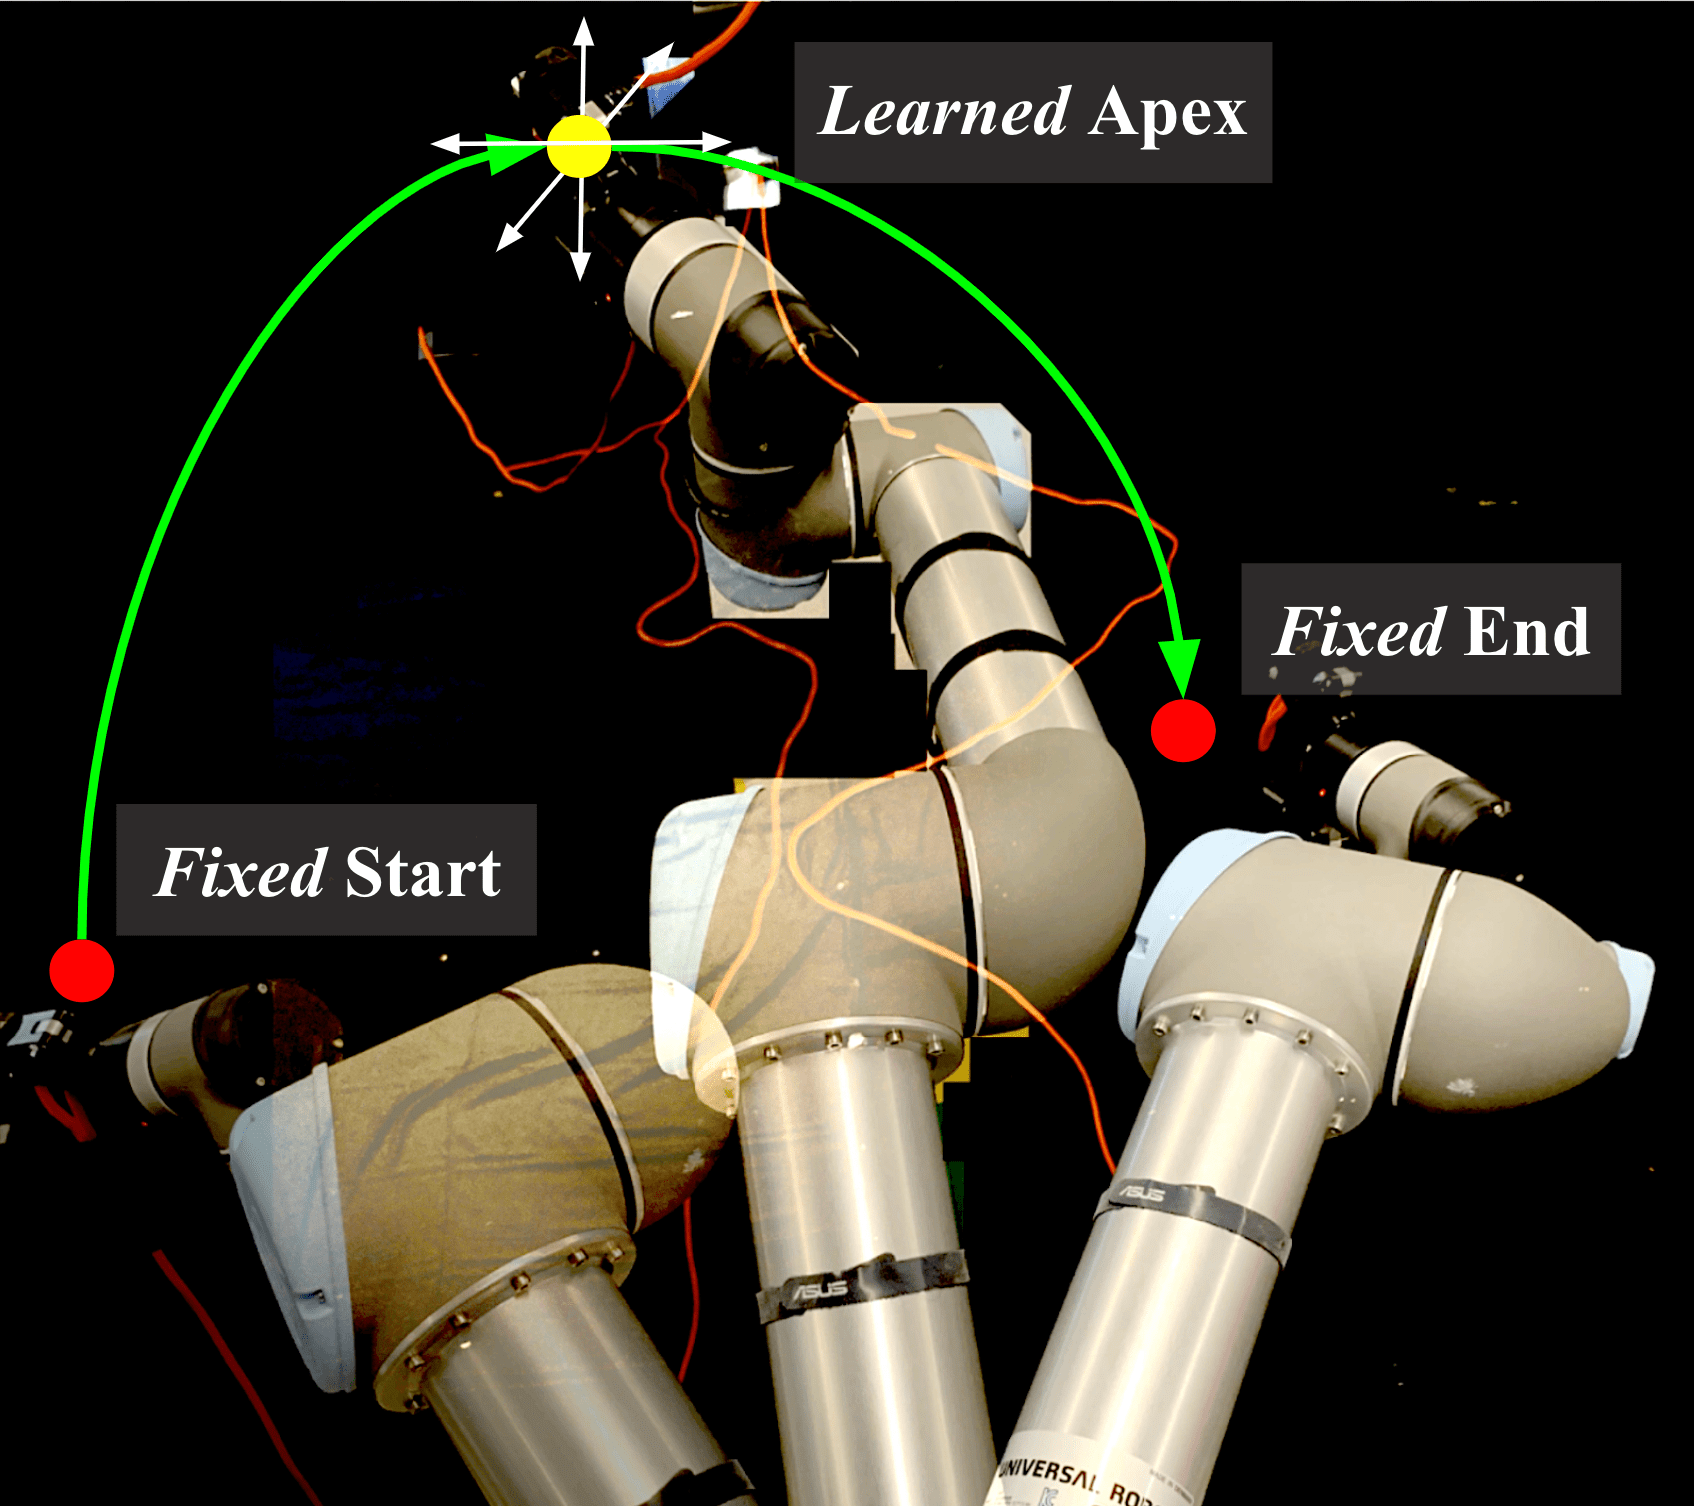
\includegraphics[width=\linewidth]{figures/3point.png}
%     \caption{Using three points in a curve to control the trajectory of the cable. The start and end points are fixed using the arm configurations. We change the trajectory by varying the apex configuration.}
%     %\vspace*{-10pt}
%     \label{fig:3point}
% \end{figure}


INDy uses a trajectory generation function $f_{\mathcal{A}_i} : \mathbb{R}^3 \rightarrow \mathcal{A}$ to reduce the output dimension of the neural network, % trained in Sec.~\ref{sec:deep_alg},
while still being able to achieve a high success rate on tasks.  In initial experiments, we observed that for the trajectory to be dynamically feasible, the trajectory generation must also limit and minimize jerk.  Otherwise, acceleration changes would often be too fast for the manipulator arm to follow while burdened by the inertia of the cable.

We propose a function based on a quadratic program (QP) that has these features and empirically achieves high success rates in the 3 tasks.  %To generate a trajectory, 
%We formulate and solve a quadratic program (QP). 
We first discretize a trajectory to $H+1$ time steps, each with $h$ seconds apart.  At each time step $t \in \irange 0H$, the discretized trajectory has a configuration $\vec{q}_t$, and a configuration-space velocity $\vec{v}_t$ and acceleration $\vec{a}_t$.  With constraints in the QP, we enforce that the trajectory is kinematically and dynamically feasible, starts and ends at 2 fixed arm configurations, and reaches an apex configurations defined by the output of the learned policy.  The objective of the QP minimizes jerk.  To make the trajectory as fast as possible, in a manner similar to GOMP~\cite{GOMP}, we repeatedly reduce $H$ by 1 until the QP is infeasible, and use the shortest feasible trajectory.  The QP takes the following form:
\begin{small}
\begin{align*}
    \argmin_{(\vec{q},\vec{v},\vec{a})_{\irange 0H}} \; & \frac 1{2h} \sum_{t=0}^{H-1} (\vec{a}_{t+1} - \vec{a}_{t})^{\intercal} Q (\vec{a}_{t+1} - \vec{a}_{t}) \\
    \text{s.t.} \; & \vec{q}_0 \text{ is the start configuration} \\
    & \vec{q}_{\lfloor H/2 \rfloor} \text{ is the apex configuration} \\
    & \vec{q}_H \text{ is at the end configuration} \\
    & \vec{v}_0 = \vec{v}_{H} = \vec{0} \\
    & \vec{q}_{t+1} = \vec{q}_t + h \vec{v}_t + \tfrac 12 h^2 \vec{a}_t \quad \forall t \in \irange 0{H-1} \\
    & \vec{v}_{t+1} = \vec{v}_t + h \vec{a}_t \quad \forall t \in \irange 0{H-1} \\
    & \vec{q}_\mathrm{min} \le \vec{q}_t \le \vec{q}_\mathrm{max} \quad \forall t \in \irange 1{H-1} \\
    & \vec{v}_\mathrm{min} \le \vec{v}_t \le \vec{v}_\mathrm{max} \quad \forall t \in \irange 1{H-1} \\
    & \vec{a}_\mathrm{min} \le \vec{a}_t \le \vec{a}_\mathrm{max} \quad \forall t \in \irange 0{H-1} \\
    & h \vec{j}_\mathrm{min} \le \vec{a}_{t+1} - \vec{a}_t \le h\vec{j}_\mathrm{max} \quad \forall t \in \irange 0{H-1}.
\end{align*}
\vspace*{-15pt}
\end{small}

%As with DJGOMP~\cite{DJGOMP}, the QP minimizes the sum of squared jerks (changes in acceleration) experienced in the joint space. 
%In physical experiments, minimizing and limiting the jerk was necessary to prevent automated E-stops due to physical motions deviating from planned high-jerk trajectories.  
The $Q$ matrix is a diagonal matrix that adjusts the relative weight of each joint.  The QP constraints, in order, fix the start, midpoint, and end configurations ($\vec{q}_0$, $\vec{q}_{\lfloor H/2 \rfloor}$, $\vec{q}_{H}$); fix the start and end velocity ($\vec{v}_0$, $\vec{v}_{H}$) to zero; enforce configuration and velocity dynamics between time steps ($\vec{q}_{t+1}$, $\vec{v}_{t+1}$); keep the joints within the specified limits of configuration ($\vec{q}_\mathrm{min}$, $\vec{q}_\mathrm{max}$), velocity ($\vec{v}_\mathrm{min}$, $\vec{v}_\mathrm{max}$), acceleration ($\vec{a}_\mathrm{min}$, $\vec{a}_\mathrm{max}$), and jerk ($\vec{j}_\mathrm{min}$, $\vec{j}_\mathrm{max}$).
%In addition, to minimize the trajectory time like GOMP, after solving the QP, we shrink the $H$ by $1$ and repeat the process until the QP is no longer solvable due to constraint violations.
Unlike GOMP, we do not consider obstacle avoidance in the trajectory generation, and instead ensure that there are no obstacles in the path of the arm to avoid.  In practice, we fix $h$ to be an integer multiple of the robot's control frequency, and the initial value of $H$ to be sufficiently large such that there is always a solution.

The input to the trajectory function constrains the midpoint configuration of the trajectory.  As most trajectories lift then lower the end effector through the midpoint, the input is often the apex of the motion.  With the UR5 robot, we observe that varying the first 3 joints (base, shoulder, elbow) moves the end-effector's location in $(x,y,z)$.  The base joint rotates left and right, while the shoulder and elbow joints lift and extend.  We thus use these 3 joints to define the midpoint, while having the remaining joint configurations depend linearly on the first three.
We make this function a task-specific function by constraining the start and end configurations to depend on the task.  For example, for the left-to-right vaulting task, we set the start configuration to be down and left, and the end configuration to be down and right.

\section{Simulatior}
\label{sec:sim2real}

We use simulation to experiment with training algorithms, and to find a feasible base action $a_\beta$ to bootstrap the data collection process in the real world.  Using simulation enables fast prototyping to efficiently assess qualitative and quantitative behavior of multiple base actions, but can suffer from a sim-to-real gap, motivating research teams to collect data from running robots in the real world~\cite{gupta2018,folding_fabric_fcn_2020}. Similarly, we collect data by running a physical UR5 robot, but use simulation as a means to obtain a functional action that can be improved upon when collecting data.

To model cables in simulation, we use a Featherstone~\cite{featherstone1984robot} rigid-body simulator from BulletPhysics via Blender~\cite{blender}. Cables consist of a series of small capsule links connected by spring and torsional forces. %spring constants, torsional stiffness, and damping coefficients that make the simulated cable behave physically similar to power cords we use in physical experiments. 
We tune the spring and torsional coefficients by decreasing bending resistance and stopping before the cable noticeably behaves like individual capsules rather than a cable, and increasing twist resistance until excessive torsion causes the capsules to separate.
%We use a 4:1 scale between simulation and real, because when the radius of the simulated cable is below 10 cm, the collision effects between capsules disconnect the cable.
%Specifically, in Blender, we use a torsional stiffness value of 1, a twist damping value of 0.9, a spring stiffness value of 40, and a spring damping value of 0.5.

When finding a feasible $a_\beta$ to transfer to real, we only simulate vaulting. The obstacle height, radius, and location are randomized for each trial, along with the initial cable state. We use 10 different obstacle and initial cable settings in simulation, and select the input apex point with highest success rate out of 60 random points. Then, we take this apex point directly to physical experiments as the base action $a_\beta$ to collect data, as the physical UR5 exhibits similar behavior to that in simulation after applying the predefined configurations from simulation, as seen in Fig.~\ref{fig:sim_to_real}.

% We use Blender~\cite{blender,priya_2020,descriptors_fabrics_2020}, as its keyframe feature allows us to specify robot configurations at certain animation frames, with the robot motion between keyframes being automatically interpolated. 

%Additionally, Blender has an easy to use Python API, and its built-in rendering engine Eevee supports ray-tracing, making rendering fast on GPUs.
% because it has previously worked reasonably well for manipulating 1D~\cite{priya_2020} and 2D structures~\cite{descriptors_fabrics_2020}.

% Using this setup, we compare the three-point arc model with different models. First, we tried regressing both apex point location and velocity explicitly, and found that regressing velocity did not improve the success rate of the vaulting task. We have also tried interpolating a straight-line motion between the points without making it arcing and found that the discontinuity in the middle causes the robot to come to a complete stop at the apex, thus reducing the energy stored for the cable to move fast enough.

\section{Physical Experiments}

% \begin{figure}[t]
%     \centering
%     {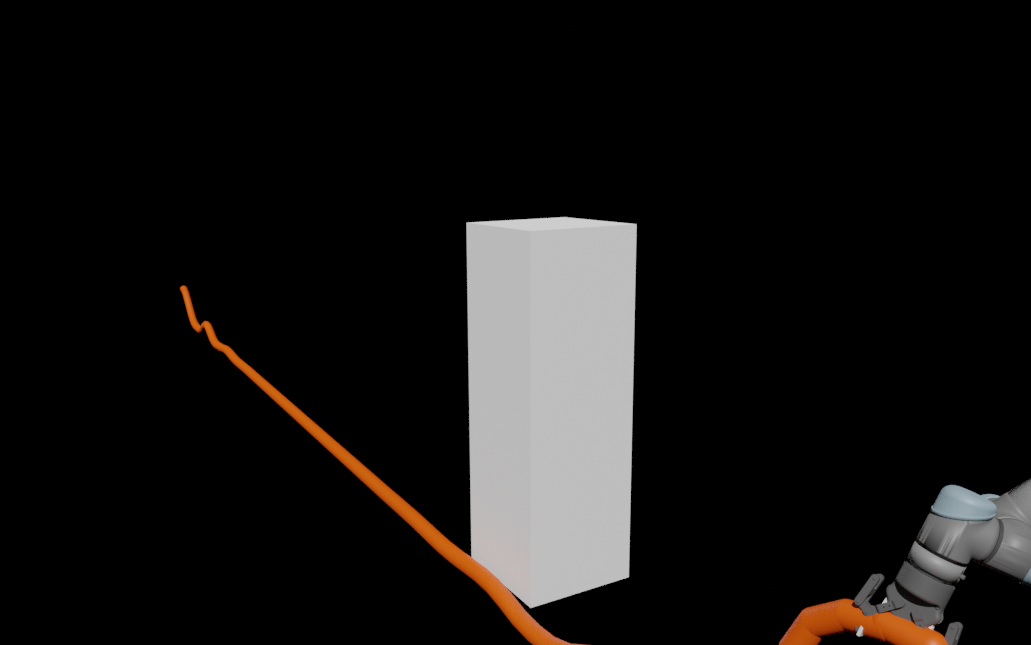
\includegraphics[width=.23\textwidth]{figures/sim_start.png}}\hfill
%     {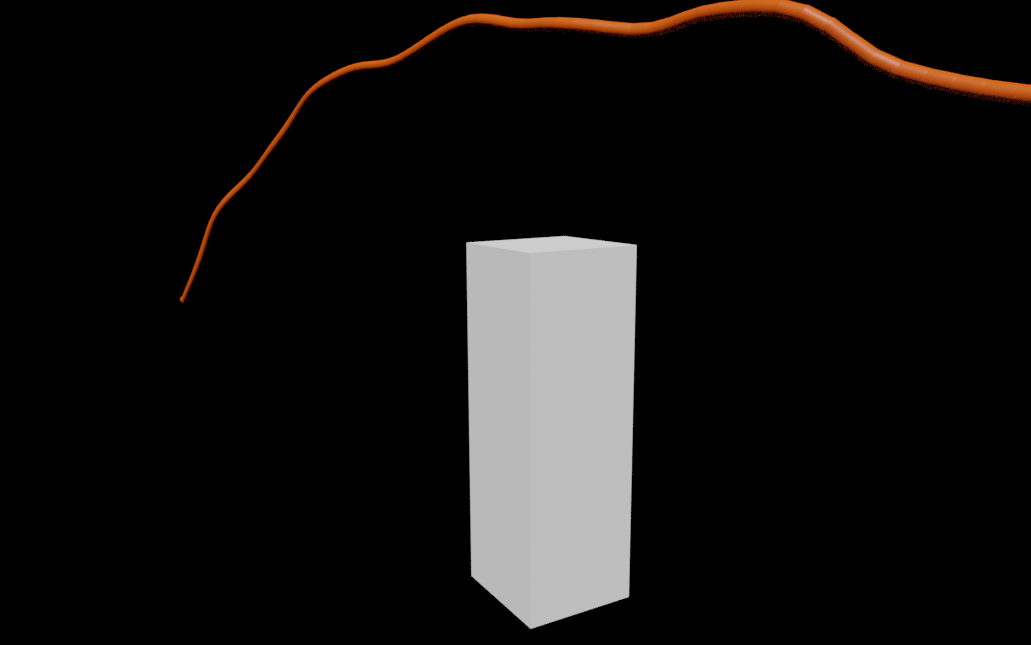
\includegraphics[width=.23\textwidth]{figures/sim_apex.png}}\hfill
%     {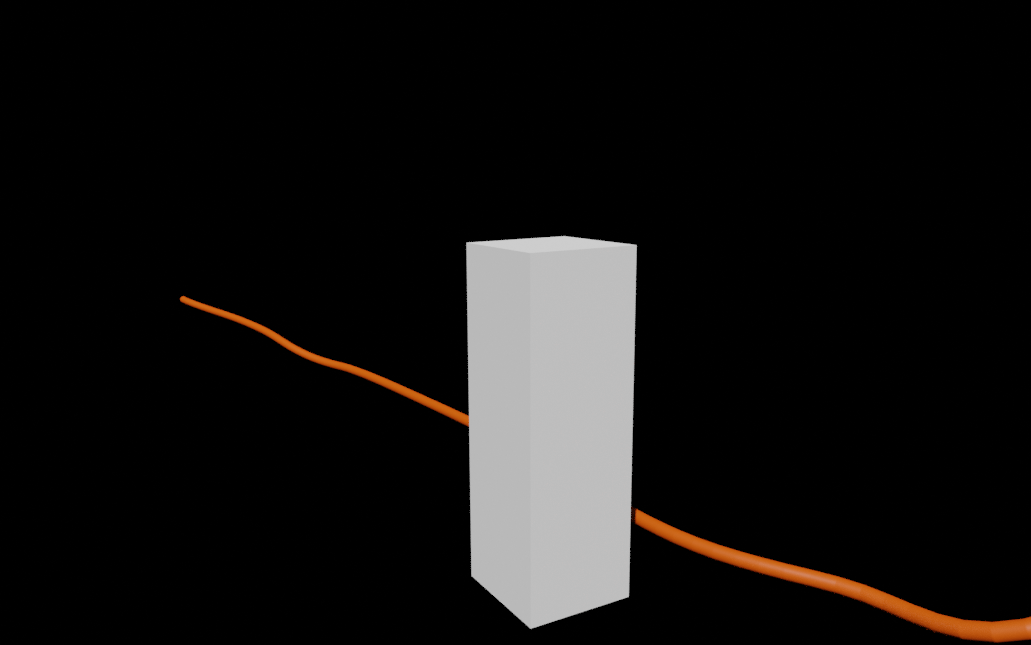
\includegraphics[width=.23\textwidth]{figures/sim_end.png}}
%     \caption{Cable trajectory for data generation in simulation (above) vs. cable trajectory in real (below) for the vaulting task.}
%     \vspace*{-10pt}
%     \label{fig:sim_to_real}
% \end{figure}
\begin{figure}
    \vspace*{5pt}
    \centering
    \begin{tabular}{@{}c@{\hspace{2.4pt}}c@{\hspace{2.4pt}}c@{}}
        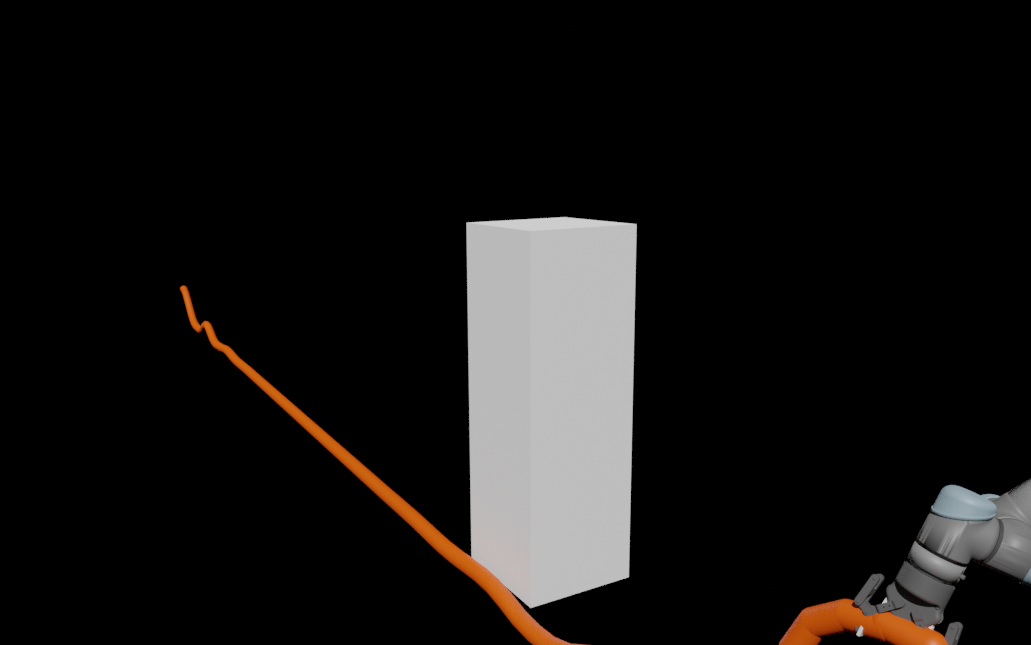
\includegraphics[width=80pt]{figures/sim_start.png} & 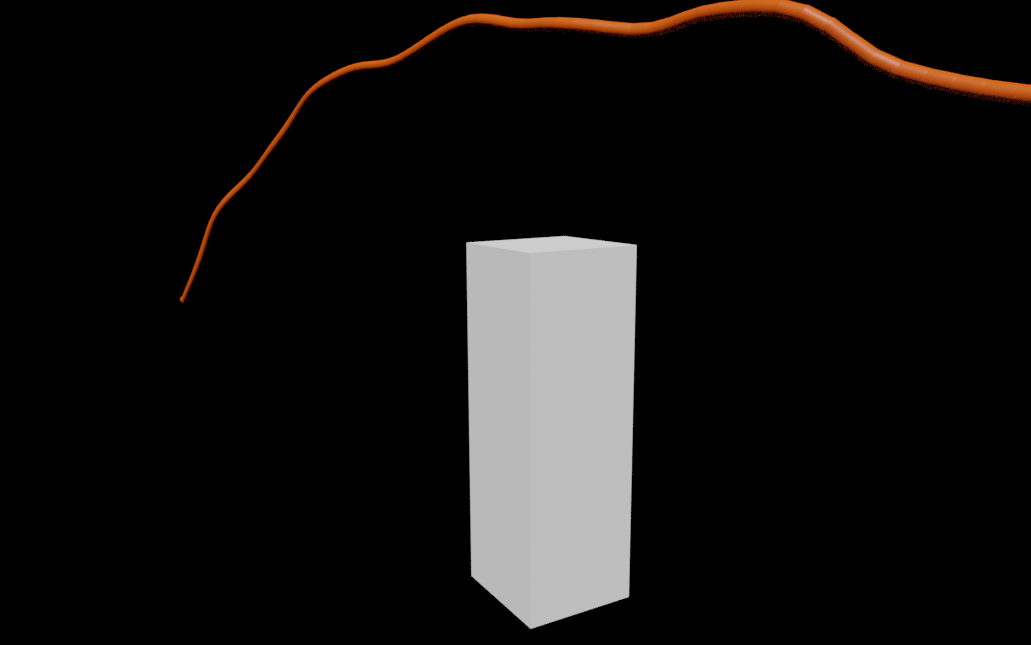
\includegraphics[width=80pt]{figures/sim_apex.png} & 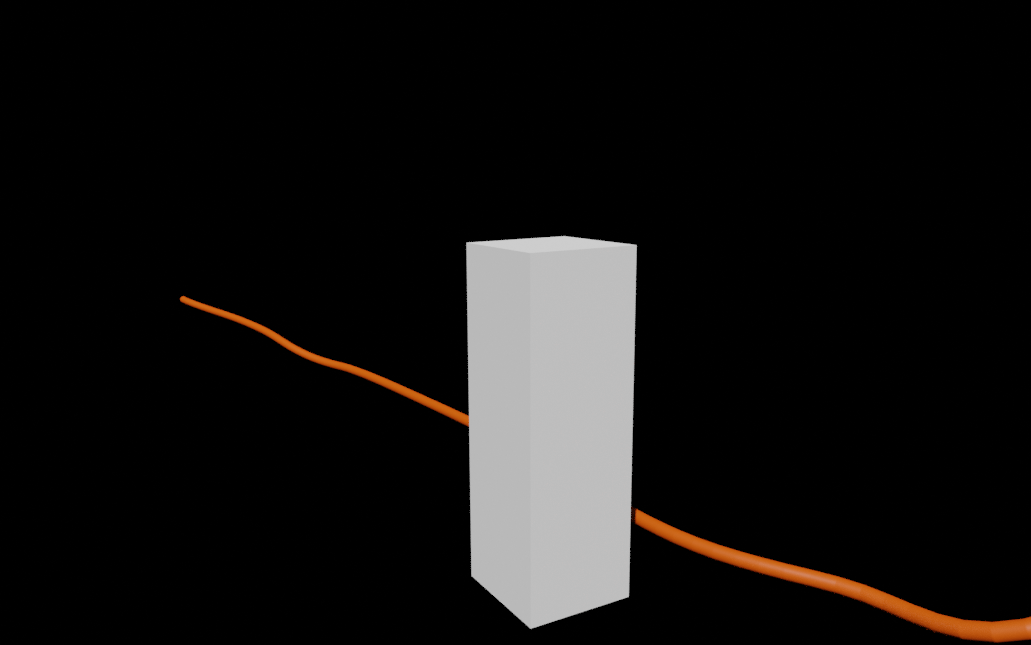
\includegraphics[width=80pt]{figures/sim_end.png} \\
        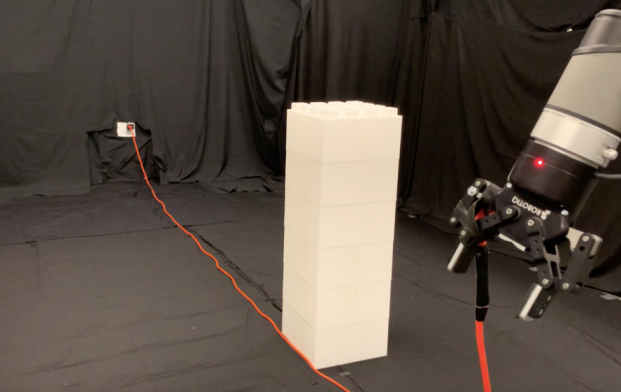
\includegraphics[width=80pt]{figures/real_end.png} & 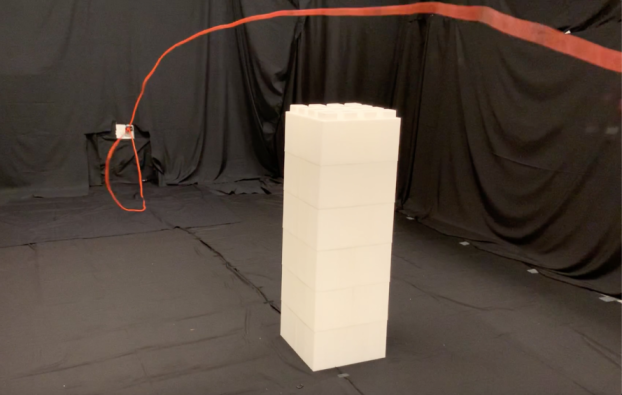
\includegraphics[width=80pt]{figures/real_apex.png} & 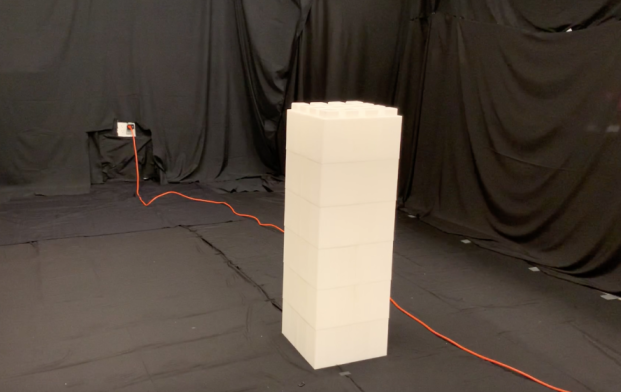
\includegraphics[width=80pt]{figures/real_start.png}\\
        \small{Start configuration} & \small{Apex configuration} & \small{End configuration}
    \end{tabular}
    \caption{Cable trajectory for data collection in \textbf{simulation (top)} vs. cable trajectory in \textbf{real (bottom)} for the vaulting task after applying the same apex point configuration.}
    \label{fig:sim_to_real}
    \vspace*{-10pt}
\end{figure}
\begin{figure}[t]
    \vspace*{5pt}
    \centering
    % \begin{tabular}{c@{\hspace{1.5pt}}c@{\hspace{1.5pt}}}
    %\subfloat[Trajectories defined by 3 points \label{fig:3point}]{%
      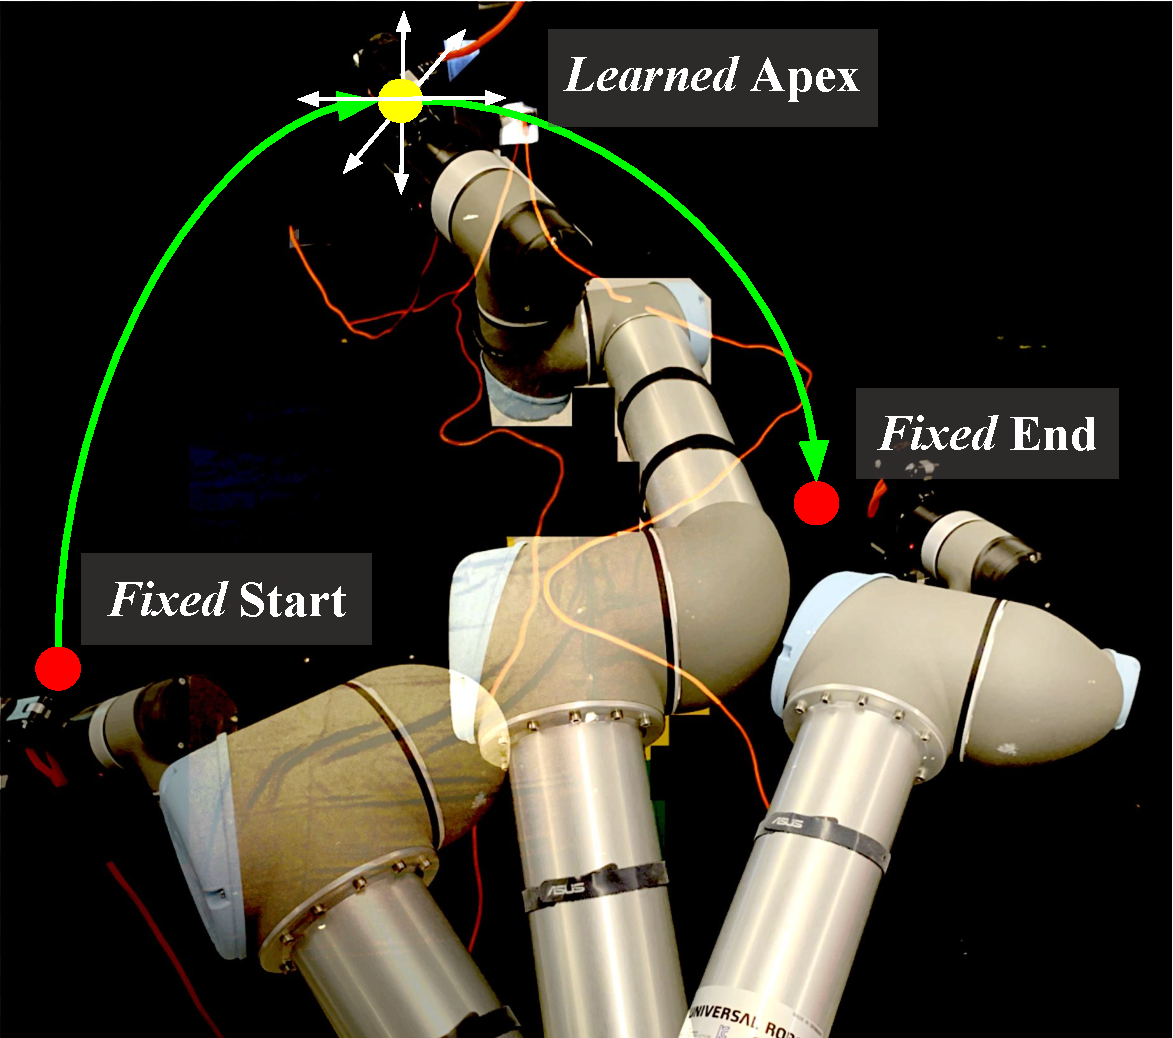
\includegraphics[height=110pt]{figures/3point.pdf}%}%
      \hfill
    %\subfloat[Physical space layout\label{fig:layout}]{%
      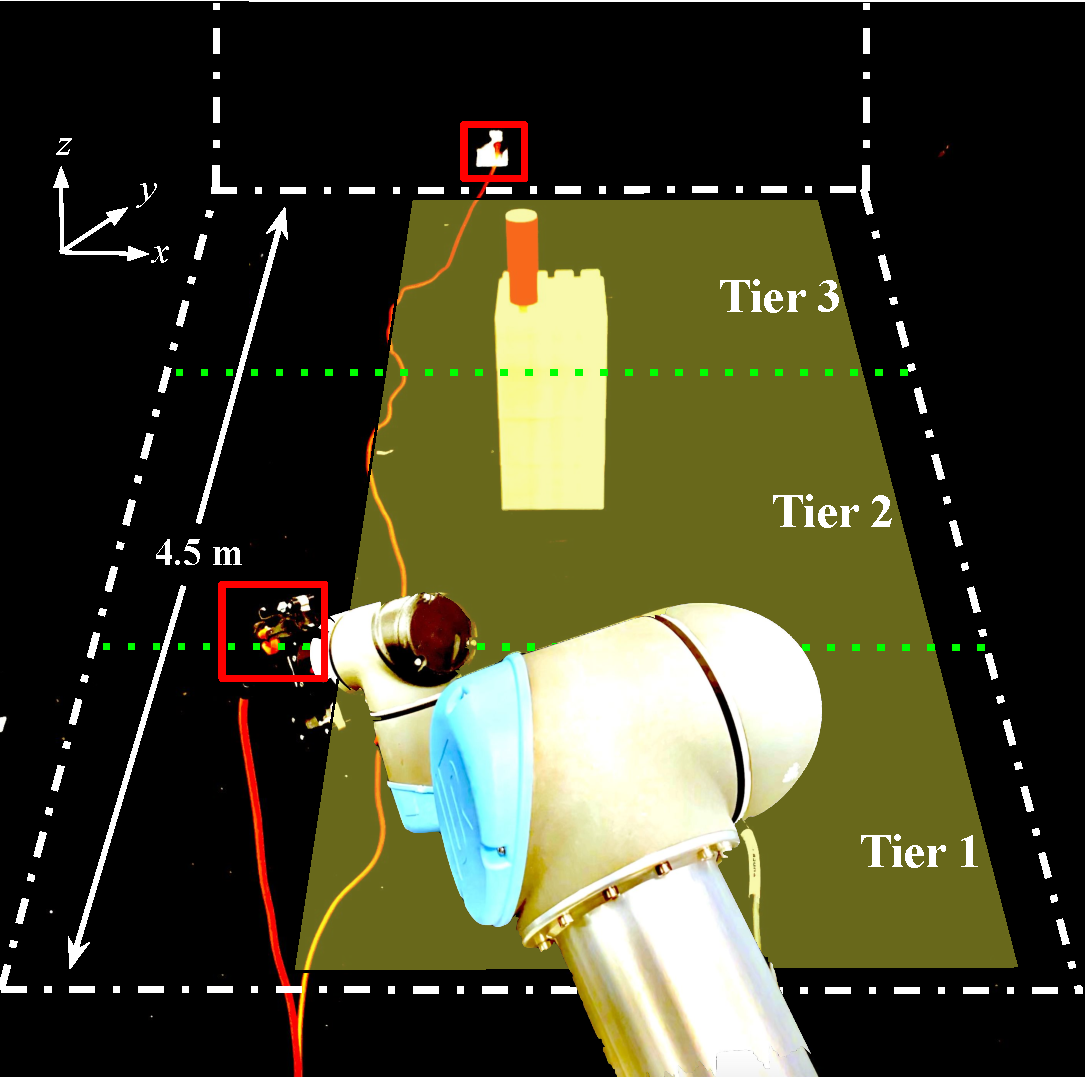
\includegraphics[height=110pt]{figures/layout_new.pdf}%}
    % \end{tabular}
    \caption{\textbf{Left: }Using three points in a curve to control the trajectory of the cable. The start and end points are fixed using the arm configurations. We change the trajectory by varying the apex configuration. \textbf{Right: }Design of physical experiments. We randomize the white Lego bricks’ location within the yellow shaded area. For vaulting and knocking, the width of the yellow area is 1.5~m, and 1.0~m for weaving. The yellow area is divided into three difficulty tiers.}
   % {\color{red} We need to change the label on the mid point.  Can you add arrows indicating that the mid point can by varied left/right and up/down (and in/out).  Also can you reverse the colors so that it starts/stops on red, and we vary the midpoint yellow.}}
    %    \vspace*{-10pt}
    \label{fig:motion_and_floor}
    \vspace*{-10pt}
\end{figure}

We use a physical UR5 robot grasping to dynamically manipulate a cable attached to a wall 4.5\,m away, on the three tasks, with 5 different cable types.
The system obtains observations from a Logitech C270 720p webcam placed 0.75\,m above the robot arm base.  It scales and crops the image to a 512x512x3 segmented RGB image that feeds into a ResNet-34~\cite{resnets_2016} deep neural network implemented with PyTorch~\cite{pytorch_neurips}.
We initialize weights using He initialization~\cite{he2015delving}.

%We use a UR5 arm on a fixed base because the arm can move fast enough to induce motions on the cable, and the fixed base allows us to control the experimental setup.
%The UR5's joints are specified to move up to 3\,rad/s, which we set as velocity constraints in the trajectory function.%, and observed the robot achieving.



%We attempted experiments on a Fetch~\cite{fetch}, but while its specification state the joints have limits in the range 1.52 to 2.27~rad/s, we found that its arm could not move quick enough to induce a similar motion on the cable.  We speculate that this may be a problem specific to the Fetch we attempted to use in our experiments.

%while the Fetch \harry{TODO: Find Fetch details.}

% \subsection{Simulation Environment}
% \jonathan{TODO: move to IV-D}
% In simulation, we compare the model that only regresses on the apex point with a model that outputs the velocity of the arm along with the apex point in the motion defined by the three points. To vary velocity of the arm in simulation, we modify the keyframe at which the arm reaches the apex point. For example, reducing the keyframe value would cause the arm to move from the start configuration to the apex point more quickly, and move from the apex point to the end configuration at a slower speed. Simulation allows for fair comparisons between our hypothesized models, as perfect resets could be done when comparing the velocity regression model to the apex point model. For simulated vaulting on randomized obstacle locations, the model that regresses both apex point location and velocity achieves a 70\% success rate, while the model that only regresses apex point location achieved a 76\% success rate. Furthermore, 27\% of the failure cases for the velocity regression model are successfully completed by the three-point model in the same setting, suggesting that simpler input is more reliable.


% \subsection{Real World Environment}
In physical experiments of the 3 tasks (see Fig.~\ref{fig:motion_and_floor} for layout),
% \begin{figure}[t]
    \centering
    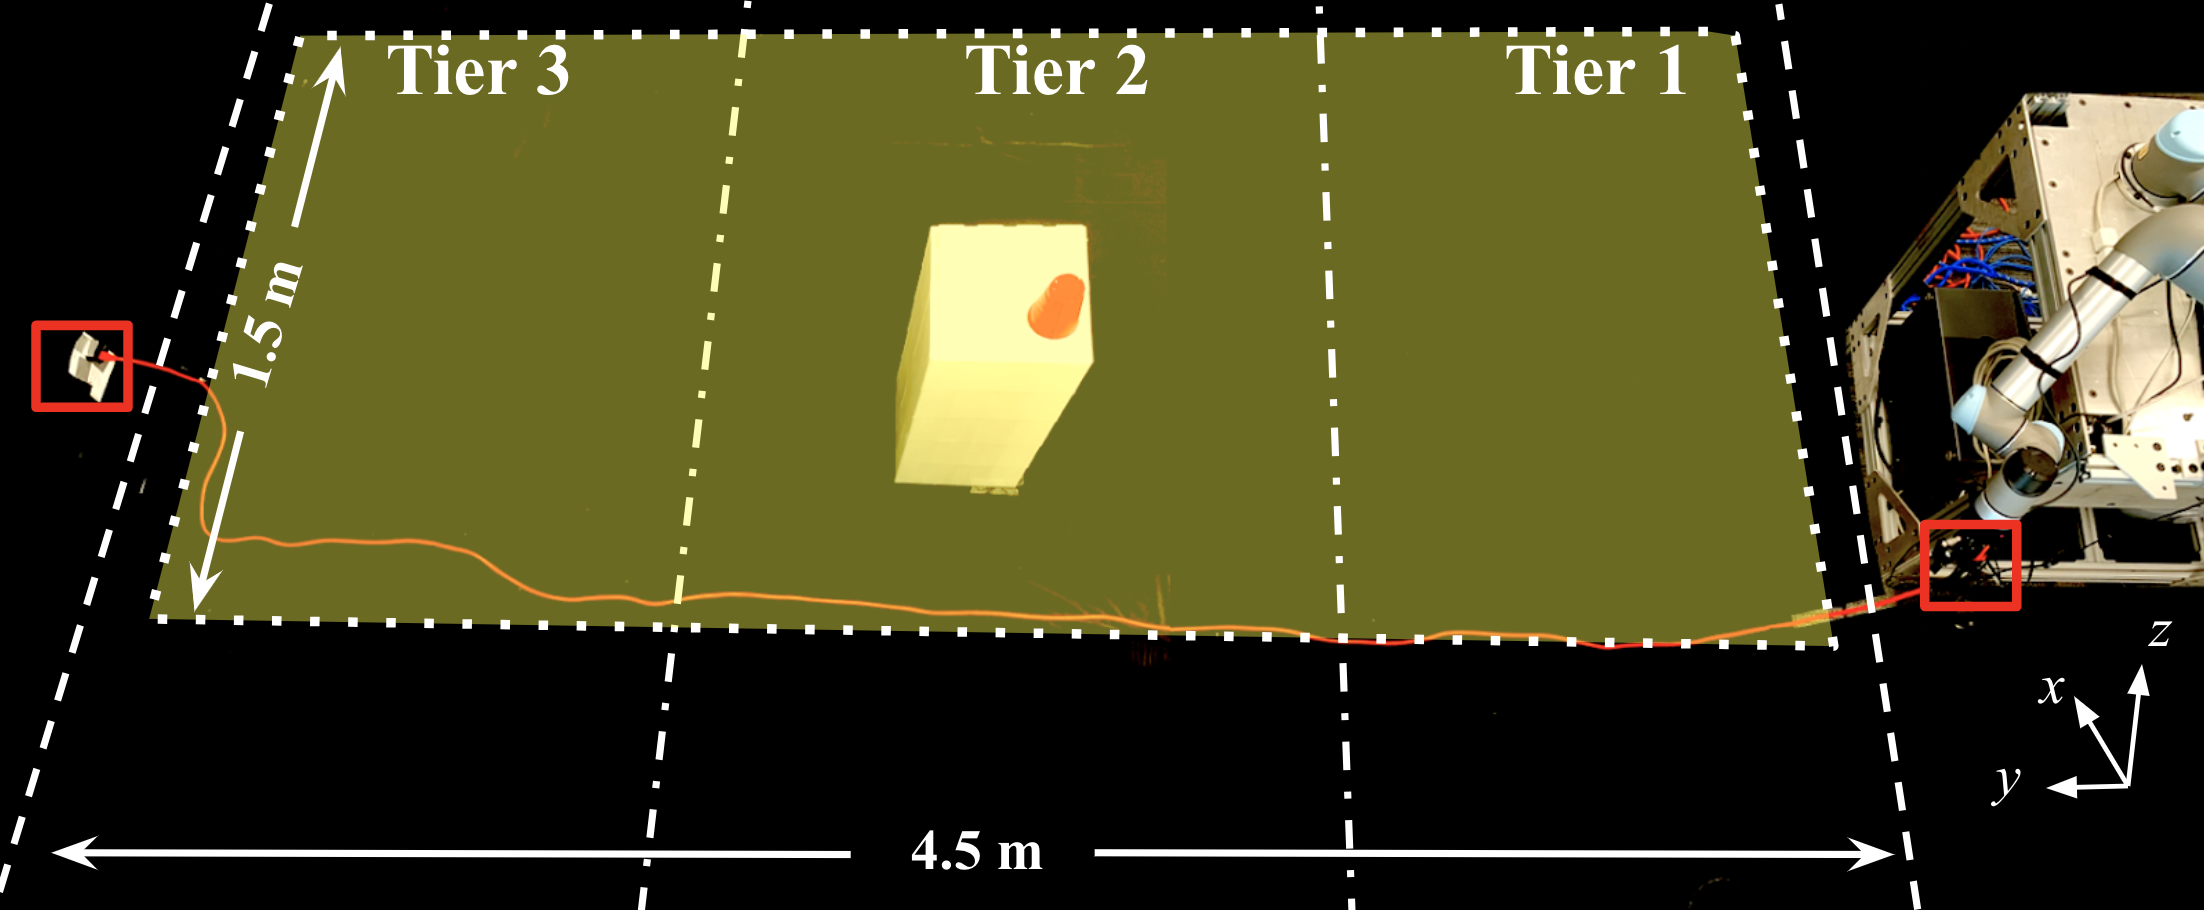
\includegraphics[width=\linewidth]{figures/layout.png}
    \caption{Design of physical experiments. We randomize the white Lego bricks' location within the yellow shaded area for vaulting and knocking. The yellow shaded area is also broken down into three difficulty tiers. Here we show an example of knocking, where the white Lego bricks form a base for the red target object on top of it and the robot aims to knock over the red target. \harry{TODO: prof. G said rotate. need to find a better way to convey the idea.}}
    \vspace*{-10pt}
    \label{fig:layout}
\end{figure}
we use large, white plastic bricks as the obstacle(s), which can vary in size and location. The obstacles we use for experiments are 0.15\,m to 0.75\,m in width and 0.3\,m to 1.5\,m in height.
To generate training data, we randomize the location and size of the obstacles in each trial.
We test the system with 5 cables listed in Table~\ref{tab:cable_types}.
%We test our system with 4 different types of cables of different lengths and calibers: a 5.5-meter orange 18-gauge power extension cable, a 5-meter white 16-gauge power extension cable, a 6.2-meter orange 14-gauge power extension cable, and a 5.5-meter blue 22-gauge ethernet cable. We also test our system on a 4.8-meter blue 12-gauge jump cable. The UR5 station's base is 4.5 meters away from the fixed end of the cable.

\begin{table}[t]
    \vspace*{4pt}
    \centering
    \caption{Physical cables used in experiments and the number of successes in the three tasks (Vaulting, Knocking, Weaving) using policies trained with the 18 AWG orange cable. For each cable, we evaluate with 20 trials for each task.}
    \begin{tabular}{@{}l@{\quad}r@{\quad}r@{\quad}r@{\quad}r@{\quad}r@{}}\toprule
        
         Type & kg & m & Vaulting & Knocking & Weaving \\
        \midrule
         18 AWG orange cable  & 0.65 & 5.5 & 16&13&12\\
         16 AWG white cable   & 0.70 & 5.2 &16&12&12\\
         16 AWG orange cable  & 0.90 & 6.2 &4&2&2\\
         22 AWG blue network cable  & 0.48 & 5.5 &14&9&12\\
         12 AWG blue jump rope   & 0.45 & 5.1 &15&10&8\\
         %5-meter white 16-gauge power extension cable, a 6.2-meter orange 14-gauge power extension cable, and a 5.5-meter blue 22-gauge ethernet cable. We also test our system on a 4.8-meter blue 12-gauge jump rope. 
         \bottomrule
    \end{tabular}
    \vspace*{-16pt}
    \label{tab:cable_types}
\end{table}

%With the starting, apex, and ending joint configurations of the robot, we feed them into the QP solver to solve for a fast, min-jerk trajectory. Once the robot executes this trajectory, we check if the trial succeeds and record data accordingly.%, where we only record the 3 joint angles of the robot at the apex of the motion when the resulting trajectory succeeds.

We define \emph{difficulty tiers} based on the distance of the obstacle to the base of the robot.
% \begin{tabular}{@{}l|l|l@{}}
%     \textbf{Tier 1: ${\pmb{\leq}}$ 1.5\,m} & 
%     \textbf{Tier 2: 1.5 to 3\,m} & 
%     \textbf{Tier 3: ${\pmb{\geq} }$ 3\,m}
% \end{tabular}
%
\begin{table}[h]
\centering
\vspace{-6pt}
\begin{tabular}{@{}ccc@{}}
    \textbf{Tier 1} & 
    \textbf{Tier 2} & 
    \textbf{Tier 3} \\
    ${\pmb{\leq}}$ 1.5\,m &
    1.5 to 3\,m & 
    ${\pmb{\geq} }$ 3\,m
\end{tabular}
\vspace{-12pt}
\end{table}
%
%
% \begin{description}
%     \item \textbf{Tier 1: ${\pmb{\leq}}$ 1.5~m} 
%     % The objects of interest are less than 1.5 meters away from the base of the robot.
%     \item \textbf{Tier 2: 1.5 to 3~m} 
%     % The objects of interest are 1.5 to 3 meters away from the base of the robot.
%     \item \textbf{Tier 3: ${\pmb{\geq} }$ 3~m} 
%     % The objects of interest are more than 3 meters away from the base of the robot.
% \end{description}
%

We evaluate INDy along with two baselines:
%
\begin{description}[align=left,leftmargin=0pt]
    \item[Baseline with Fixed Apex.] In the three tasks, for each configuration, a human annotator sets one set of apex joint angles that can accomplish the task. The apex joint angles are fixed with respect to the obstacle itself, and they remain the same across different locations of the same obstacle.
    \item[Baseline with Varying Apex.] In vaulting and weaving, for each configuration (including obstacle size and location), a human annotator sets the apex joint angles such that the robot arm's end effector is 15\,cm above the center of mass (COM) of the obstacle, and aligned horizontally with the COM of the obstacle. For knocking, a human annotator makes the robot arm end 10\,cm above the COM of the target object, and aligned horizontally with the COM.
\end{description}

We find the baselines from simulation, where we observe that the fixed and varying apex motions could induce enough velocity to make the cable vault the obstacle.
\section{Results}

% \begin{figure}[t]
% \center
% 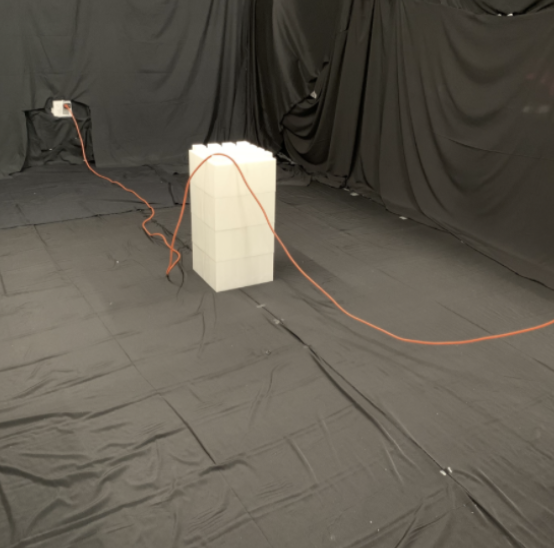
\includegraphics[width=34mm]{figures/failure.png}
% \caption{
% \small
% Failure case example. In this shown example, when the cable is too long (too slack), the motion that would have succeeded on a shorter cable fails to accomplish Task 1, and the resulting cable terminal configuration is not on the other side (right) of the obstacle, and instead the cable lands on the obstacle.
% }
% %\vspace*{-10pt}
% \label{fig:failure}
% \end{figure}
\begin{figure}[t]
    \vspace*{15pt}
    \centering
    % \begin{tabular}{c@{\hspace{1.5pt}}c@{\hspace{1.5pt}}}
    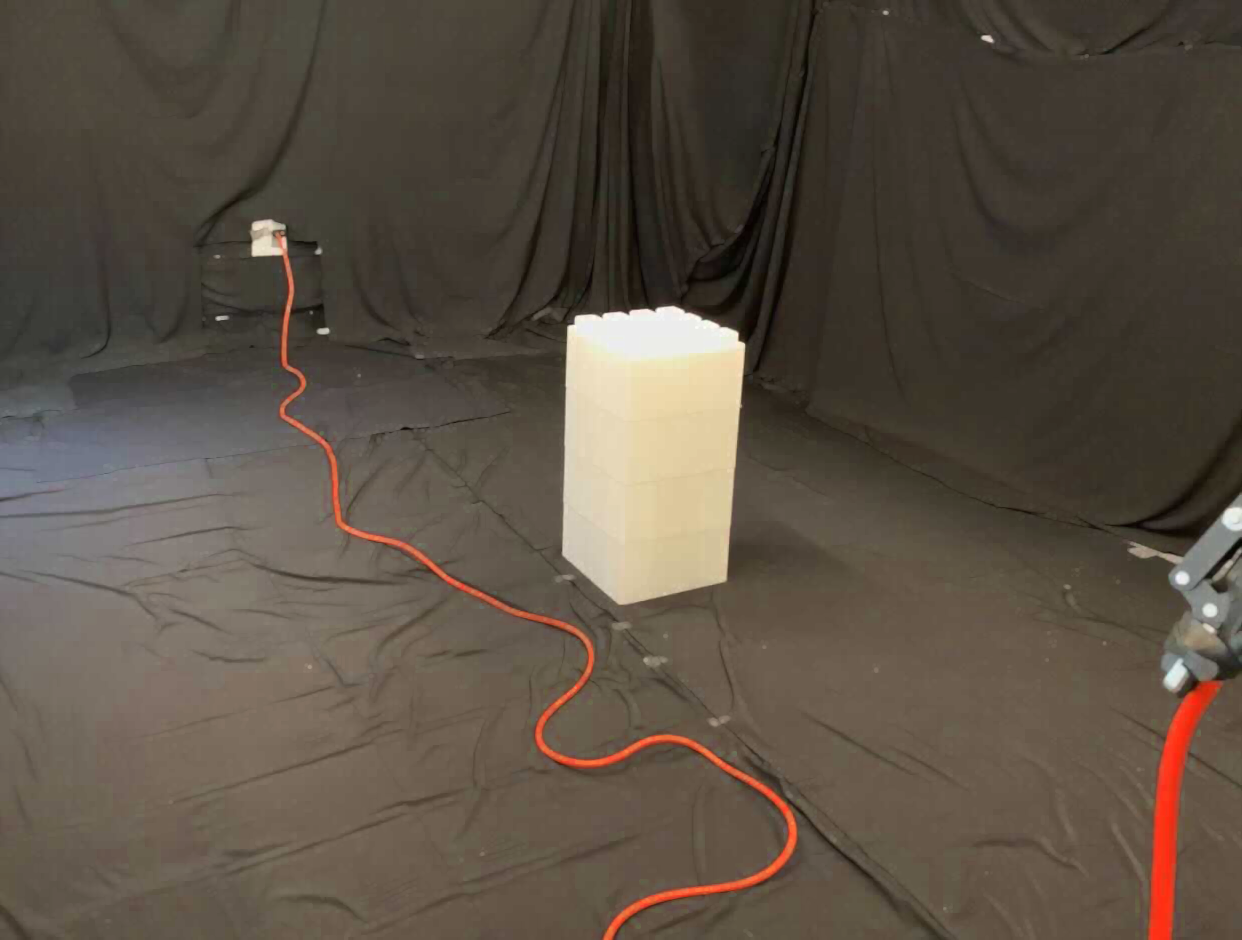
\includegraphics[width=120pt]{figures/failure_b4.png}\hfill
    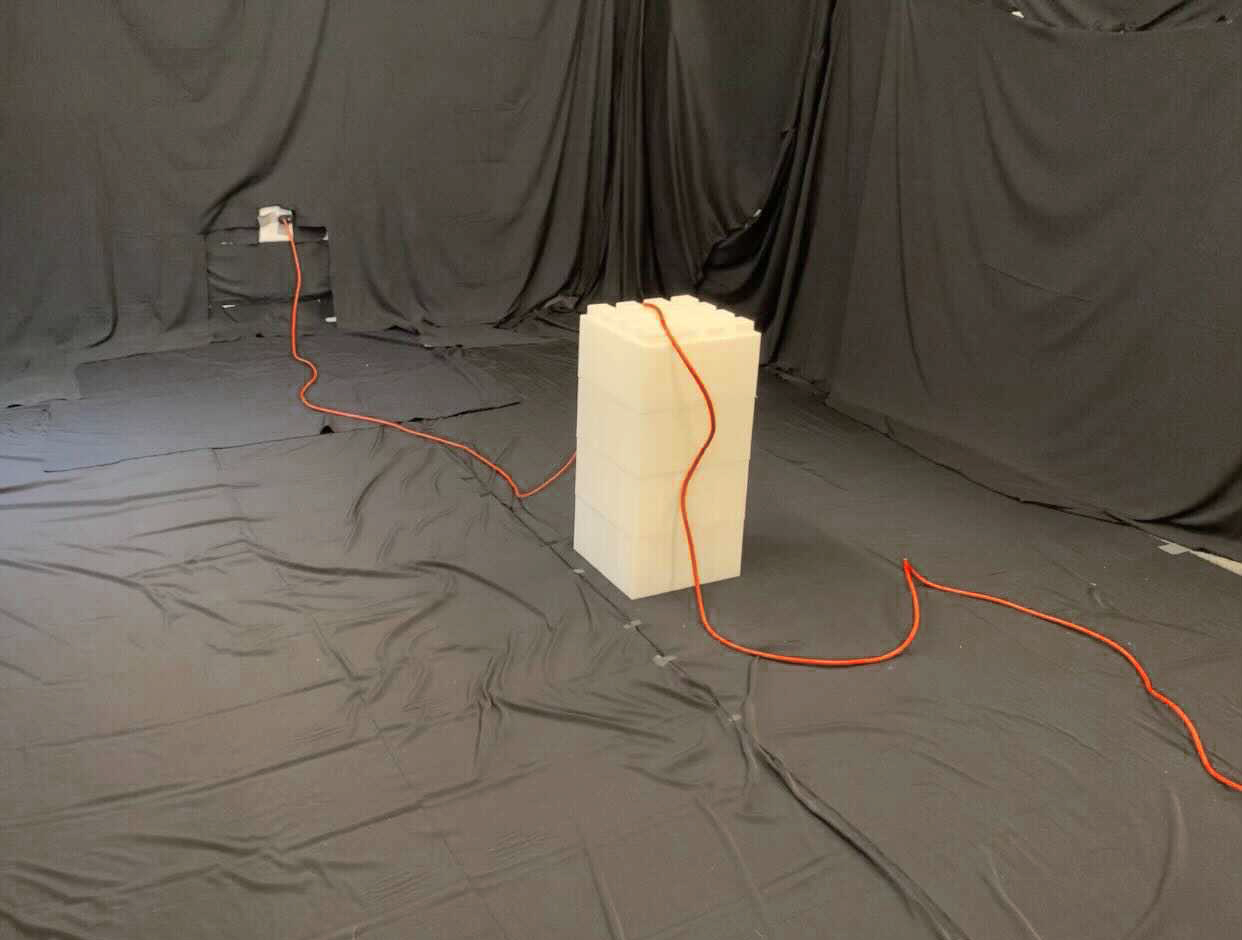
\includegraphics[width=120pt]{figures/failure_2.png}
    % \end{tabular}
    \caption{\textbf{Failure mode}. The 16-gauge 6.2~m orange cable is too long for the vaulting motion.  \textbf{Left:} before the motion there is too much slack. \textbf{Right:} the vaulting motion that works for shorter cables does not clear the obstacle.} %and the resulting cable terminal configuration is not on the other side (right) of the obstacle, and instead the cable lands on the obstacle.}
    
    \label{fig:failure}
\end{figure}

% The results suggest the learned policies can generalize to a variety of settings in terms of the objects' shapes and locations. 

We measure the correlation between simulated and real setups, benchmark the three dynamic cable tasks, and investigate generalization to different cables. %Across vaulting, knocking, and weaving, the learned apex procedure outperforms the baselines with fixed and varying apexes by 31.5\% and 16.5\%. 
%Since dynamic cable manipulating is best understood in action, We recommend viewing the supplementary videos on the project website.
The project website supplements these results with videos.

\subsection{Comparisons between Simulation and Reality}

To observe correlations between cable behavior in simulation and real, we evaluate vaulting on the same set of apex point and obstacle settings in both setups. Each trial consists of a random obstacle location from all 3 difficulty tiers and a different apex point. In simulation, we use a cube mesh of the same dimension as the plastic bricks obstacle in real, and a cable of the same length and mass as the 18 AWG orange cable. Table~\ref{table:sim_to_real} reports the frequency of success and failure cases across simulation and real. While the cable trajectory in simulation tends to match the trajectory of real for successes, 50\,\% of all failed cases in real succeed in simulation under the same setting. The discrepancies in cable behavior between simulation and real are most apparent for Tier 3 scenarios, where the height achieved by the cable at the opposite end from the robot differ in the two environments.  Because the cable properties cannot be perfectly tuned to match the physical properties in real, these experiments motivate the decision to use real experiments to collect data.
% 9 success cases and 6 failure cases from real are evaluated in the same conditions in simulation.

% \begin{tabular}{l|l|c|c|c}
% \multicolumn{2}{c}{}&\multicolumn{2}{c}{Real}&\\
% \cline{3-4}
% \multicolumn{2}{c|}{}&Successes&Failures&\multicolumn{1}{c}\\
% \cline{2-4}
% \multirow{2}{*}{Simulation}& Successes & $a$ & $b$\\
% \cline{2-4}
% & Failures & $c$ & $d$\\
% % \cline{2-4}
% % \multicolumn{1}{c}{} & \multicolumn{1}{c}{Total} & \multicolumn{1}{c}{$a+c$} & \multicolumn{    1}{c}{$b+d$} & \multicolumn{1}{c}{$N$}\\
% \end{tabular}

% \begin{table}
%     \vspace*{5pt}
% \centering
% \caption{Success rates of different vaulting apex points performed in simulation and real across 15 trials.}
% {    
% \begin{tabular}{cc|ccc}
% \multicolumn{2}{c}{}
%             &   \multicolumn{2}{c}{Real} \\
%     &   match   & differ &   Success &   Failure              \\ 
%     \cline{2-4}
% % \rotatebox[origin=c]{90}{Simulation}
%     Simulation
%     & Success   & 46.67\%&20\%\\
%     & Failure    & 13.33\%&20\%\\ 
%     \cline{2-4}
%     \end{tabular}
%     \vspace*{-10pt}
%  }
%  \label{table:sim_to_real}
% \end{table}
 
 \begin{table}
    \vspace*{4pt}
\centering
\caption{Number of successes and failures for vaulting in simulation and physical environments across 15 trials, evaluating a different apex point on a different obstacle position for each trial. Listed are the number of cases that succeed in both sim and real, fail in sim but succeed in real, succeed in sim but fail in real, and fail in both sim and real. The correlation between success rates in the two environments is surprisingly high.}
%\vspace{0.3cm}
 \begin{tabular}{ 
l c c}
% \multicolumn{4}{c}{Task 1 Results}\\
 \toprule
   & \#Success (Simulation) & \#Failure (Simulation) \\
  \midrule
  \#Success (Physical)&7&2\\
  \#Failure (Physical)&3&3\\
 \bottomrule
\end{tabular}
\vspace*{-5pt}

\label{table:sim_to_real}
\end{table}
\subsection{Results for Vaulting Task}
For vaulting, we perform 180 physical trials from manipulating the orange 5.5\,m 18-gauge power extension cable, with 60 trials for each of the 3 difficulty tiers; this process took 8 hours. In each tier, we shift the obstacle vertically within the bounds of the difficulty tier and horizontally within a range of 1.5\,m. We use plastic bricks to construct 6 combinations to build 6 objects of different sizes, and for each obstacle, we vary its location 10 times. Table~\ref{table:res_task1} shows results of the trained policy on vaulting evaluated with 20 trials per tier.

\begin{table}[t]
\vspace*{0pt}
\centering
\caption{Physical Vaulting Results: Number of successes of the learned policy for vaulting evaluated against two baseline methods across 20 trials per difficulty tier using the 18 AWG orange cable.}
%\vspace{0.3cm}
 \begin{tabular}{ 
l c c c}
% \multicolumn{4}{c}{Task 1 Results}\\
 \toprule
  Method & Tier 1 & Tier 2 & Tier 3\\
  \midrule
  Baseline with Fixed Apex&16&13&2\\
  Baseline with Varying Apex&19&14&7\\
  Learned Apex &\textbf{20}&\textbf{18}&\textbf{11}\\
 \bottomrule
\end{tabular}

\label{table:res_task1}
\end{table}

% For this task, we also evaluate the reversed-direction vaulting motion without training on the reversed-direction data. We reflect the input image and feed it into the network to plan a motion. It turns out we can accomplish reversed vaulting without actually training on reversed direction data. Intuitively, this is because since we are only regressing the midpoint (apex) of the motion, and we fix the starting and ending configurations of the robot, which are almost mirrored, the learned policy should be agnostic to the direction of vaulting. We achieve 100\% success in Tier 1, 80\% in Tier 2, and 50\% in Tier 3.
% Note that the result is slightly worse because the robot is not positioned perfectly in the center (slightly to the right), so the learned apex point is also conditioned on that center location.

\subsection{Results for Knocking Task}

For knocking, we perform 180 physical trials from manipulating the orange 5.5-m 18-gauge power extension cable, with 60 trials for each of 3 difficulty tiers; this process took 9 hours. In each difficulty tier, we use the plastic bricks as the base upon which we place the target object to be knocked, and we shift the plastic bricks base vertically within the bounds of the difficulty tier and horizontally within a range of 1.5\,m. We train the policy using four different target objects: a cylinder, a tennis ball, a cup, and a rectangular box. We use plastic bricks to construct 3 combinations to build 3 bases of different sizes. For each base, we vary its locations 5 times, and for each location of the base, we vary the target on top 4 times. 
%We also collect additional 30 trials using Hindsight Experience Replay (HER)~\cite{andrychowicz2017hindsight} in order to fully utilize the data. After we train with the 180 trials, we test the trained policy and collect all the failure cases where the cable lands on the Lego base but does not hit the object of interest. We take an image of the reset scene with the object placed at the location on the base where the cable landed and pretend that the object would have been hit successfully if it had been placed there, and the regression label remains the same as in the failure case. With these 30 additional trials, we finetune the trained network. 
Table~\ref{table:res_task2} shows the results for the knocking trained policy evaluated with 20 trials for each difficulty tier.% is shown in Table~\ref{table:res_task2}.
\begin{table}
\vspace*{4pt}
\centering
\caption{Physical Knocking Results: Number of successes of the learned policy for knocking evaluated against two baseline methods across 20 trials per difficulty tier using the 18 AWG orange cable.}
%\vspace{0.3cm}
 \begin{tabular}{ %p{2.8cm}||p{1cm}|p{1cm}|p{1cm}|p{1cm} | p{1cm}| p{1cm}| p{1cm}| p{1cm}|p{1cm}}
l c c c}
% \multicolumn{4}{c}{Task 2 Results}\\
 \toprule
  Method & Tier 1 & Tier 2 & Tier 3\\
  \midrule
  Baseline with Fixed Apex &12&6&4\\
  Baseline with Varying Apex &14&14&6\\

  Learned Apex&\textbf{15}&\textbf{14}&\textbf{10}\\
 \bottomrule
\end{tabular}
\label{table:res_task2}
\end{table}

\subsection{Results for Weaving Task}

We perform 100 physical trials from manipulating the orange 5.5-m 18-gauge power extension cable, which took 7.5 hours. We make the 3 obstacles identical in size. In our training data for this task, we vary the space between each object by 15 to 50\,cm and we shift the obstacles horizontally within a range of 1\,m.
%We evaluate weaving task by checking if the policy can produce two actions that manipulate a cable to be weaved between three objects. 
Table~\ref{table:res_task3} shows the result of the weaving trained policy evaluated with 20 trials. % is shown in Table~\ref{table:res_task3}.
% \begin{figure}
%     \vspace*{5pt}
%     \centering
%     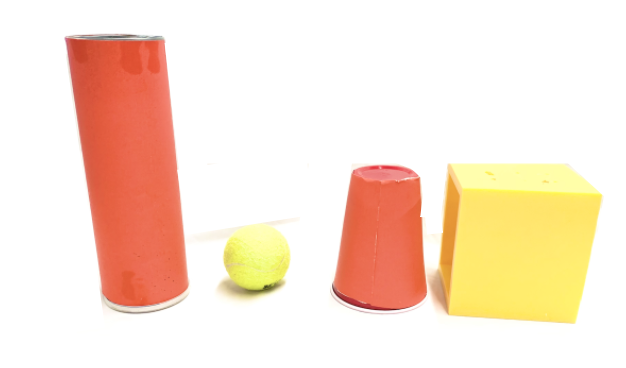
\includegraphics[width = 0.3\linewidth]{figures/targets.png}
%     \caption{Target objects used for training the knocking policy}
%     \label{fig:targets}
%     \vspace*{-10pt}
% \end{figure}

\subsection{Generalization to Different Cables}
%{\color{red} TODO: Add more details for each task and include number of trials per KG 10/29} 
While the policies for the three tasks are trained using the 18-gauge orange cable, we experiment with different types of cables. The results suggest that the policy trained on the 18-gauge orange cable can transfer well to other cables of similar lengths. We observe that the same reset action can bring these cables to nearly identical starting configurations in observation space, making the policy agnostic to cable type. We use the learned policy from the 18-gauge orange cable without retraining or finetuning to run the same experiments (same object sizes and locations for each task) for the 3 tasks with different cables and show results in Table~\ref{tab:cable_types}. 
%Using the 5.2-meter white 16-gauge cable, we achieve 80\% success rate for vaulting, 60\% success rate for knocking, and 60\% success rate for weaving. With the 5.5~m 22-gauge ethernet cable, we achieve 80\% success rate for vaulting, 50\% success rate for knocking, and 60\% success rate for weaving. With the 4.8~m 12-gauge jump rope, we achieve 80\% success rate for vaulting, 50\% success rate for knocking, and 40\% success rate for weaving.
\begin{table}
%\vspace*{-10pt}
\vspace*{0pt}
\centering
\caption{Physical Weaving Results: Number of successes of the learned policy for weaving evaluated against two baseline methods across 20 trials using the 18 AWG orange cable.}
%\vspace{0.3cm}
 \begin{tabular}{ %p{2.8cm}||p{1cm}|p{1cm}|p{1cm}|p{1cm} | p{1cm}| p{1cm}| p{1cm}| p{1cm}|p{1cm}}
l c c c}
% \multicolumn{4}{c}{Task 2 Results}\\
 \toprule
  Method & \#Success\\
  \midrule
  Baseline with Fixed Apex &3\\
  Baseline with Varying Apex &3\\

  Learned Apex&\textbf{12}\\
 \bottomrule
\vspace*{-10pt}
\end{tabular}
\label{table:res_task3}

\end{table}
\vspace*{-8pt}
\subsection{Limitations and Failure Modes}

While the framework can be robust to object locations and shapes, it has limitations. First, the policies are learned in a highly controlled environment. % where we constrain obstacles to a relatively small area.
Many failure cases in vaulting and knocking are from %outliers of 
placements outside the training area. For example, in Tier 3 vaulting, 7 of 9 failure cases are due to the horizontal shift of the obstacle exceeding the 1.5\,m bound. In weaving, the horizontal shift of the obstacles is bounded into a smaller 1.0\,m range.%so the trained weaving policy would not generalize to a variety of obstacles settings.
%
% Starting a paragraph with "Second," seems weird, unless we have a paragraph that starts with "First,"
Second, learned policies have difficulty generalizing to cables of different lengths and masses. We conjecture that with different lengths, the amount of slack in the cables should also be different, thus decreasing the repeatability of applying the same action. With the 6.2\,m cable, Tier 2 and 3 vaulting and knocking always fail in that the segment of the cable near the wall end can never be accelerated up due to the fact that the slack near the wall end cannot be eliminated by the resetting action.
%We hypothesize that this is the case because when the cable is too long, it would require more energy to be accelerated, and the energy generated from the action output by the policy trained on a shorter cable is lower than the expected energy, thus failing to manipulate the longer cable as desired. 
To show this failure mode with a longer cable, we run the policies for vaulting, knocking, and weaving trained with the 5.5-m 18-gauge cable on the 6.2-m 16-gauge cable, and we achieve 20\,\% success rate for vaulting, 10\,\% success rate for knocking, and 10\,\% success rate for weaving. Fig.~\ref{fig:failure} shows this failure case. Additionally, Table~\ref{tab:cable_types} suggests that cables that are too light are likely to yield lower success rates, which may be because they often travel slower during descent, limiting the distance the cable traverses. Finally, the data generation part in Alg.~\ref{alg:whip} is inefficient since when the obstacle size and location change, the algorithm needs to search for successful apex point again, so data generation in real is unable to record a wider variety of obstacle placements in an efficient manner.

% Lastly, our experiment environment is a highly controlled one and the obstacles and target objects we have used are fairly simple. More variations in the environment should be expected in real-life scenarios such as different obstacles and different target objects. To make the proposed system applicable in real life, we would need to collect more data from a variety of different obstacles and target objects or apply heavy domain randomization techniques to make the policy generalizable and we leave this to future work.


\section{Conclusion}

This paper explores learning three dynamic cable manipulation tasks:  vaulting, knocking, and weaving. Experimental results suggest that the proposed procedure outperforms two baseline methods.

In future work, we will generalize the learned policy to different cable lengths and masses, and more complex obstacles and target objects. We will apply the parameterized trajectory method to other dynamic cable manipulation tasks without fixed-endpoints of the cable, inspired by the adventures of Dr. Indiana Jones.
%As we experiment with dynamic motions of the cable manipulation, we think there could be a mathematical relation between the joint apex configuration and the cable's landing location that does not need to be learned by a CNN, and we are currently investigating the relation by observing the data. We will also investigate meta deep reinforcement learning-based controllers that allow us to learn a wider variety of tasks. We are also working on accomplishing tasks where the endpoints of the cable are not fixed, and extending the proposed system to tossing motions.
% and fabric~\cite{rishabh_2020,seita_fabrics_2020} manipulation.



\section{Acknowledgments}

\footnotesize
This research was performed at the AUTOLAB at UC Berkeley in
affiliation with the Berkeley AI Research (BAIR) Lab, the CITRIS ``People and Robots'' (CPAR) Initiative, and the Real-Time Intelligent Secure Execution (RISE) Lab. The authors were supported in part by donations from Toyota Research Institute and by equipment grants from PhotoNeo, NVidia, and Intuitive Surgical. Daniel Seita is supported by a Graduate Fellowship for STEM Diversity (GFSD). We thank our colleagues who provided helpful feedback, code, and suggestions, in particular Francesco Borrelli, Adam Lau, Priya Sundaresan, and Jennifer Grannen.

% Daniel: I just noticed, if you set IEEEtran as the bibliography, references appear in the order they are cited, but IEEEtranS (with the 'S' at the end) means references appear in alphabetical order. I advocate for alphabetical order.
\bibliographystyle{IEEEtran}
\bibliography{IEEEabrv,references}

\clearpage
% \normalsize
% \onecolumn
% \appendix
\section{Appendix}
\label{sec:appendix}
The appendix is organized as follows:

\daniel{TODO insert extra text here}

\end{document}
